\documentclass{article}
\usepackage[final]{neurips_2021}

\usepackage[utf8]{inputenc} % allow utf-8 input
\usepackage[T1]{fontenc}    % use 8-bit T1 fonts
\usepackage{hyperref}       % hyperlinks
\usepackage{url}            % simple URL typesetting
\usepackage{booktabs}       % professional-quality tables
\usepackage{amsfonts}       % blackboard math symbols
\usepackage{nicefrac}       % compact symbols for 1/2, etc.
\usepackage{microtype}      % microtypography
\usepackage{xcolor}         % colors
\usepackage{lipsum}
\usepackage{amsmath}
\usepackage{setspace}
\usepackage{bbm}
\usepackage[linesnumbered,ruled,commentsnumbered]{algorithm2e}
\usepackage{parskip}
\usepackage{graphicx}
\usepackage{caption}
\usepackage{subcaption}

\graphicspath{
  {./figures/active/neural/}
  {./figures/active/linear/}
  {./figures/online_similarity/linear/}
  {./figures/online_similarity/neural/}
}

\IncMargin{1.5em}

\title{Active Heirarchical Metric Learning}

\author{
  Nicolas Beltran\\
  Department of Computer Science\\
  Columbia University\\
  New York City, NY 10027 \\
  \texttt{nb2838@columbia.edu}\\
  \And
  Ketan Jog\\
  Department of Computer Science\\
  Columbia University\\
  New York City, NY 10027 \\
  \texttt{kj2473@columbia.edu}\\
}


\begin{document}

\maketitle

\begin{abstract}
    Many problems require a well defined notion of a distance between points in space.
    Constructing or finding such a measure falls into the field of metric learning.
    Although many algorithms exist in the field when a learner has access to a fixed dataset,  there is room for improvement in terms of samples efficiency that the learner needs to know, imposition of desired structure, especially when the data appears in an \textit{online} manner.
    We propose a project that reduces the problem of online/active metric learning to bandits. In case our plan turn out to be too ambitious, we have a fallback - an empirical investigation of some algorithms that have dealt with the problem in an online setting or in situations where the learner can selective query the points that it wants to know information about.
\end{abstract}


\section{Introduction}

\section{Related Work}

\section{Long-term goals}

\section{Preliminaries}


% --------------------------------------------------------------
% --------------------------------------------------------------
\section{Problem Statement}
\label{problem-statement}
% --------------------------------------------------------------
% --------------------------------------------------------------
We consider two different problems.
The first problem consists of making a series of sequential predictions while learning a
similiarity measure. We refer to this problem as online similarity prediction.
The second problem consists of learning a similarity measure while querying points in space.
We refer to this problem as active similarity learning.

\subsection{Online similarity learning}
\label{problem-statement:online-similarity-learning}
We consider an online similarity learning problem played over $T$ rounds.
At round $t$ the environment samples $K$ pairs of points $(x_{t,k}, y_{t,k}) \in \mathbb{R}^{2n}$.
The agent then chooses pair $k_t \in [K]$ and is given a reward $r_{t,k_{t}} \in \{1, -1\}$.
We assume that there exists some similarity function unknown to the agent $\phi: \mathbb{R}^{2n} \to \{-1, 1\}$
and that the rewards are such that if at time $t \in [T]$ the agent chooses pair $(x_{t,k}, y_{t,k})$
then the reward is $\phi(x_{t,k}, y_{t,k})$.

As usual we define the regret as
\[ R_T = \mathbb{E}\left[\sum_{t =1}^T \phi(x_{t,k^\star_t}, y_{t,k^\star_t}) - \phi(x_{t,k_t}, y_{t,k_t})\right]\]
where $k_t^\star = \text{argmax}_{k\in [K]} \phi(x_{t,k}, y_{t,k})$

\subsection{Active similarity learning}
\label{problem-statement:active-similarity-learning}
We assume that the learner has access to a dataset $D = \{x_i \in \mathbb{R}^n| i \in [N]\}$ of unlabeled points and that there exists some function $\phi: \mathbb{R}^{2n} \to \{-1, 1\}$ which the learner is trying to learn.
The learner can query $T$ pairs of points in this set $D$ to obtain a dataset $D_T = \{(x_t, y_t, r_t) ~|  ~t \in [T]\}$  where $x_t$ and $y_t$ are the points in space and $r_t$ is their similarity.
The learner mantains and estimate $\hat{\phi}_t \in \mathcal{F}$ of $\phi$, where $\mathcal{F}$ is its function class and we denote the loss between an estimate $\hat{\phi}$ a $\phi$ as
\[ \mathcal{L}(\phi, \hat{\phi}) = \mathbb{E}_{(x, y) \sim \mathcal{D} \times \mathcal{D}}[(\hat{\phi}(x,y) - \phi(x, y))^2] \]
In this problem the goal is to find $\min_{\phi \in \mathcal{F}} \mathcal{L}(\hat{\phi}_T, \phi)$.


\section{Description of the algorithms}
We provide 4 algorithms  which can be grouped into neural and linear bandit version. We refer to our algorithms as OnSim-LinUCB, ActSim-LinUCB,OnSim-NeuralUCB, ActSim-NeuralUCB, depeding on whether the bandit algorithm they are based on and the probelm
they are trying to solve. The algorithms are all very similar but we provide them in full for completeness.


\subsection{Online similarity learning}
\subsubsection{OnSim-LinUCB}
By assuming a linear structure in the similarity function, our first algorithm performs a straighforward reduction of the online learning problem to that of regular contextual linear bandits as described in \cite{linucb}.
Mathematically, we model the similarity of two points as  $\phi(x, y) = x^\top A y$.
This is reasonable if we consider that
\[\phi(x, y) = x^\top A y = \sum_{i =1}^n\sum_{j=1}^n x_i y_j A_{i,j} \]
which we is linear in $A$ and thus allows us to use the framework of LinUCB for our problem.
The algorithm can be found in the appendix in \ref{algo:onsim-linucb}. We omit it from the main text due to its similarity with the first algorithm in \cite{linucb}.


\subsubsection{OnSim-NeuralUCB}
The expressive power of the above framework is quite limited because of the fact that Algorithm \ref{algo:onsim-linucb} assumes that similarity is the result
of a dot prouct in which both points are independently mapped to a new representation via a linear transformation. This will obviously not be true for many datasets.
To overcome these limitations we adapt NeuralUCB \cite{neuralucb} to our circumstances.

Formally, we assume that
\[ \phi(x,y) = \cos\left(f(x;\mathbf{\theta}), f(y;\mathbf{\theta})\right) = \frac{\langle f(x;\mathbf{\theta}), f(y;\mathbf{\theta}) \rangle}{||f(x;\mathbf{\theta})||_2 ||f(y;\mathbf{\theta})||_2}\]
\footnote{It is also possible to assume that we don't normalize the last inner product, we refer to this verision and unormalized NeuralUCB. We provide some comparisons of this verison also below.}
Here $f: \mathbb{R}^n \to \mathbb{R}^m$ is a simple neural network of the form
\[ f(x; \theta) = b_L + W_{L} \sigma\left(b_{L-1} +  W_{L-1} \sigma\left( \dots \sigma\left(b_1 + W_1 x\right)\right) \right)\]
for some $L \in \mathbb{N}_{\geq 2}$, $W_1 \in \mathbb{R}^{d \times n}$, $W_{L} \in \mathbb{R}^{m \times d}$, $W_{l} \in \mathbb{R}^{d\times d}$ if $l \in [2, L-1]$, $b_L \in \mathbb{R}^m$, $b_l \in \mathbb{R}^d$ for $l \neq L$, and where $\sigma(x) = \max\{0, x\}$ applied component wise. We use $\theta$ to denote the flattened vector of $(W_L, b_L, \dots, W_1, b_1)$.
Using this notation OnSim-NeuralUCB is described below in Algorithm \ref{algo:onsim-neuralucb}. We use $p$ to denote the total number of trainable parameters in the neural network.

\begin{algorithm}
  \setstretch{1.2}
    \SetKwInOut{Input}{Input}
    \Input{Rounds $T$, exploration parameter $\alpha$, $\tau_r$ frequency of resets, $\tau_T$ frequency of training, $E$ epochs for training, $b_s$ batch size for training, $\epsilon$ learning rate.}
    $A \gets I_{p}$\;
    \For{$t \in [T]$}{
      Observe $K$ pairs of vectors $x_t^k \in \mathbb{R}^n$, $y_t^k \in \mathbb{R^n}$\;
      \For{$k \in [K]$}{
        $p_{t,k} \gets \phi(x,y) + \alpha \sqrt{(\nabla_\theta \phi(x_t^k, y_t^k))^\top A^{-1}\nabla_\theta\phi(x_t^k,y_t^k)}$\;
      }
      Choose pair $k_t = \text{argmax}_k p_{t,k}$ with ties broken arbitrarily\;
      Observe payoff $ r_t \in \{-1,1 \}$\;
      \If{$t \mod \tau_r = 0$ }{
        $\theta \gets \text{Train}(\epsilon,E, \{(x_i^{k_i}, y_i^{k_i}, r_i)\}_{i=1}^t,b_s)$\;
      }
      \If{$t \mod \tau_T = 0$ }{
        $A \gets I_p$
      }
      $A \gets A + \nabla_\theta \phi(x_t^k, y_t^k)(\nabla_\theta\phi(x_t^k,y_t^k))^\top$\;
    }
    \caption{OnSim-NeuralUCB}\label{algo:onsim-neuralucb}
  \end{algorithm}
Intuitively, this algorithm acts optimally with the current set of parameters with a bonus for exploration, and every so often it stops back to train the network.
``Train" can be found in the appendix as \ref{algo:train} but it simply describes the normal process of training a neural network with MSE loss.

Our algorithm is very similar to that proposed in \cite{neuralucb} but it differs in the following aspects: 1. We adopt a siamese neural network architecture unlike the paper.
2.We add bias 3.We use cosine similarity function in our last layer 4. We restart the the matrix $A$ after every $t \mod \tau_T = 0$ iterations 5.We use a constant exploration parameter.
We propose these changes because we believe they are more sensible for our particular application (and do provide better empirical performance) but they destroy any theoretical guarantees.
In \cite{neuralucb} these assumptions alongside arguments related to the  neural tangent kernel matrix \cite{neuraltangentkernel} are used to provide a $\tilde{O}(\sqrt{T})$, bound on the regret of algorithm.


  \subsection{Active Similarity Learning}
  Despite the differences with online similarity learning, for the active version of the problem we modify the above algorithms only slightly.
  The idea is to use the optimism bonus as a measure of uncertainty and ignore completely the reward.


  \begin{algorithm}
  \setstretch{1.2}
    \SetKwInOut{Input}{Input}
    \Input{Queries $T$, exploration parameter $\alpha$, $\tau_r$ frequency of resets, $\tau_T$ frequency of training, $E$ epochs for training, $b_s$ batch size for training, $\epsilon$ learning rate.}
    $A \gets I_{p}$\;
    \For{$t \in [T]$}{
      Sample $K$ pairs of vectors $x_t^k \in \mathbb{R}^n$, $y_t^k \in \mathbb{R}^n$ from dataset $D$\;
      \For{$k \in [K]$}{
        $p_{t,k} \gets \alpha \sqrt{(\nabla_\theta \phi(x_t^k, y_t^k))^\top A^{-1}\nabla_\theta\phi(x_t^k,y_t^k)}$\;
        \label{change:active-neuralucb}
      }
      Choose pair $k_t = \text{argmax}_kp_{t,k}$ with ties broken arbitrarily\;
      Query label $ r_t \in \{-1,1\}$\;
      \If{$t \mod \tau_r = 0$ }{
        $\theta \gets \text{Train}(\epsilon,E, \{(x_i^{k_i}, y_i^{k_i}, r_i)\}_{i=1}^t,b_s)$\;
      }
      \If{$t \mod \tau_T = 0$ }{
        $A \gets I_p$
      }
      $A \gets A + \nabla_\theta \phi(x_t^k, y_t^k)(\nabla_\theta\phi(x_t^k,y_t^k))^\top$\;
    }
    \caption{Active-NeuralUCB}\label{algo:active-neuralucb}
  \end{algorithm}

Using this framework, each time we have to make a query we can sample a subset of points in the unlabeled dataset $D$  and then we reveal the label of the pair with the highest uncertainty as measured by the bonus.
We emphasize that $r_t$ now references a label rather than a reward.
Algorithms \ref{algo:active-neuralucb} and \ref{algo:active-linucb} describe these processes formally.
In Algorithm \ref{algo:active-neuralucb} the most important change is line \ref{change:active-neuralucb} and in algorithm
\ref{algo:active-linucb} the most important change is line \ref{change:active-linucb}.

\section{Empirical Evaluation}
Below we describe the set of experiments that we performed.
We test separately NeuralUCB and LinUCB based algorithms as we logically expect them to perform
very differently due to the limitations of a linear approach.



\subsection{NeuralUCB}
\paragraph{Dataset}
Although we tested on various datasets we found the costs to train on non-toy datasets prohibitive for the neural version of the algorithms.
As a result, we mainly tested on toy datasets and provide results only for the famous crescent moons dataset an implementation of which can
be found
\href{https://scikit-learn.org/stable/modules/generated/sklearn.datasets.make_moons.html}{here}.
We also provide results on MNIST dataset in section (\ref{sec:additional-experiments}).

\paragraph{Neural Network}
For our experiments we used a 3 layer neural network with 25 hidden units in each layer and an output dimension of 2.
In addition to the description of the algorithm provided above, we also added a dropout layer after each regular layer of the neural network with
$p =0.3$.

\paragraph{Optimizer}
We attempted to use SGD, Adam, and SGD with momentum with various different hyper parameters.
Generally, We found that Adam was the best performing optimizer followed by SGD with momentum.
We used a learning rate of 0.001,a momentum of 0.9, and the default hyperparemeters in \cite{adam}.

\paragraph{Additional Parameters}
We sampled ten datapoints at time for both the online and active version of the problem. Neural networks were trained after 100 queries (or timesteps)
and trained for two epochs. Every 4 epochs we reset the matrices to their orignal states. We rotate the the data the algorithm sees every two time steps.
The values reported for losses and accuracy are computed on a heldout set of the data of 1000 datapoints.

\subsubsection{Experiment 1: Effectiveness of a linear classifier on learned features}
To determine the quality of our embeddings we used an SVM to classify the learned features and observe these values
per iteration. We report the results both for SGD with momentum and Adam. Additionally, we also report the performance of NeuralUCB
using the unormalized version of cosine similarity. All graphs contain the mean and a 95\% confidence interval
computed over 10 runs of the algorithm. The results are shown in Figures (\ref{fig:svm-non-normalized-ci}) and (\ref{fig:svm-normalized-ci})

% add figures
\begin{figure}[!h]
  \centering
  \begin{minipage}{.45\textwidth}
    \centering
    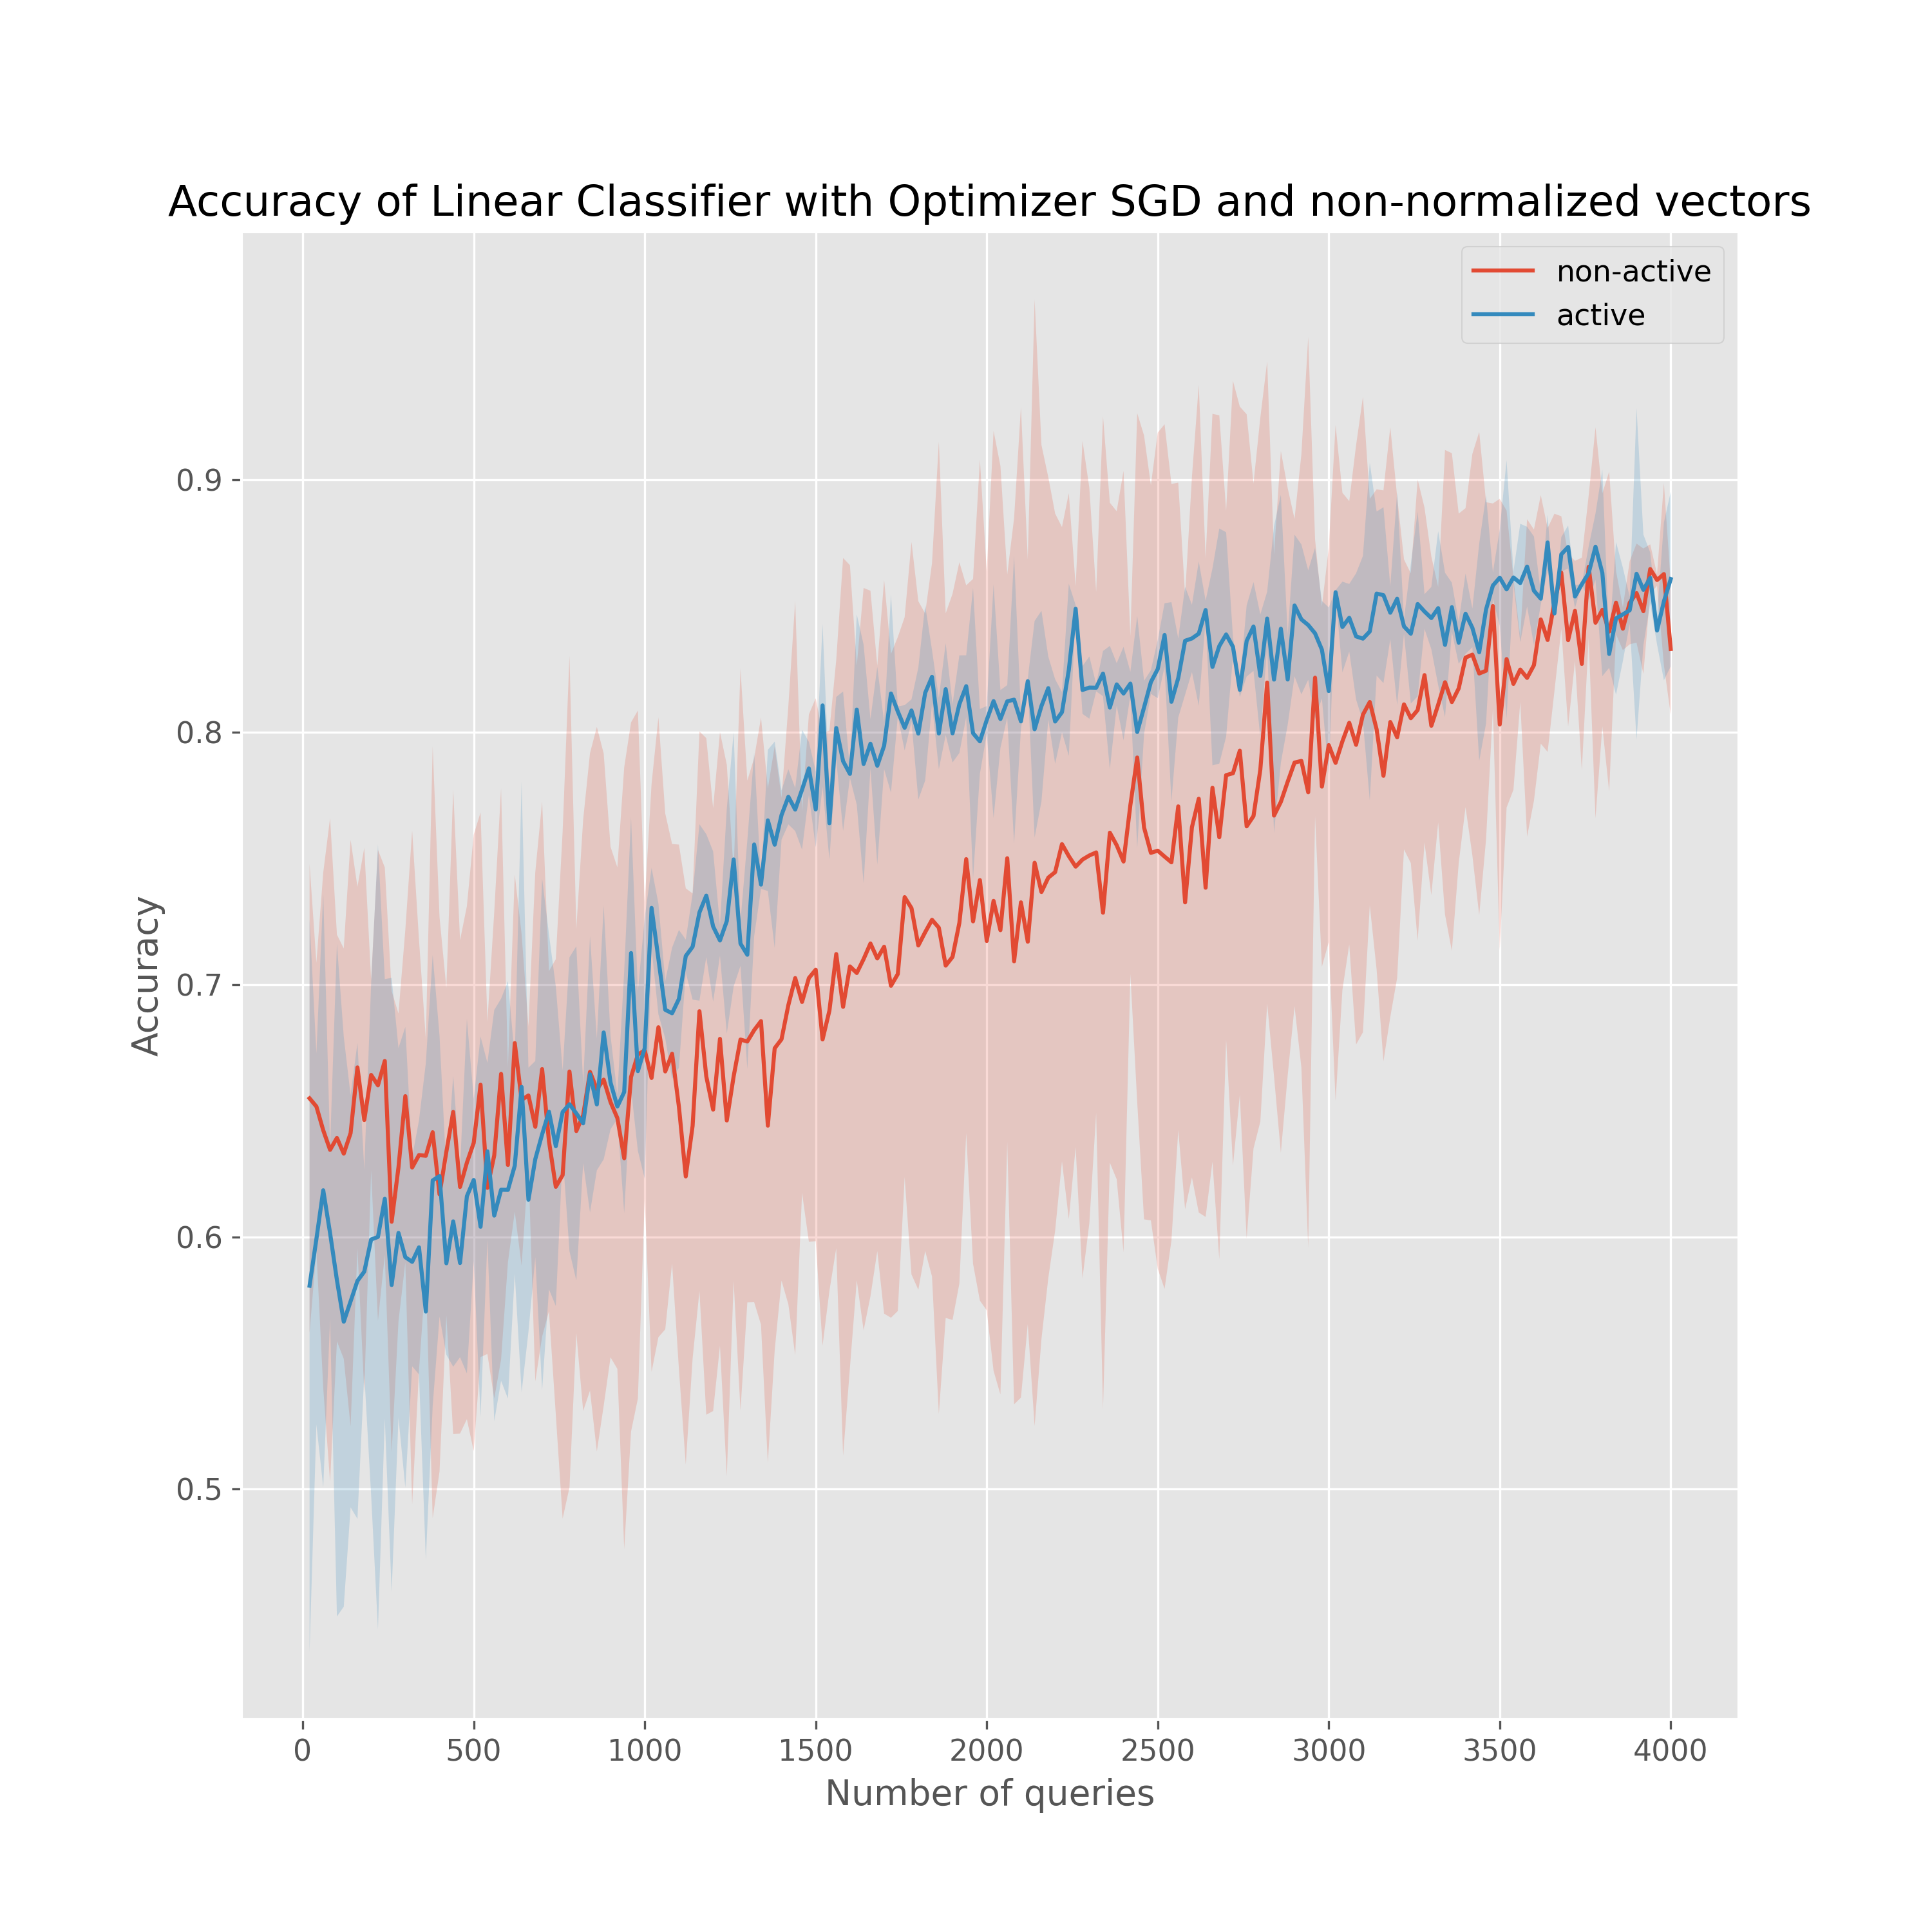
\includegraphics[width=\linewidth]{active-vs-base-moons-linear-loss-SGD-non-normalized-ci}
  \end{minipage}%
  \begin{minipage}{.45\textwidth}
    \centering
    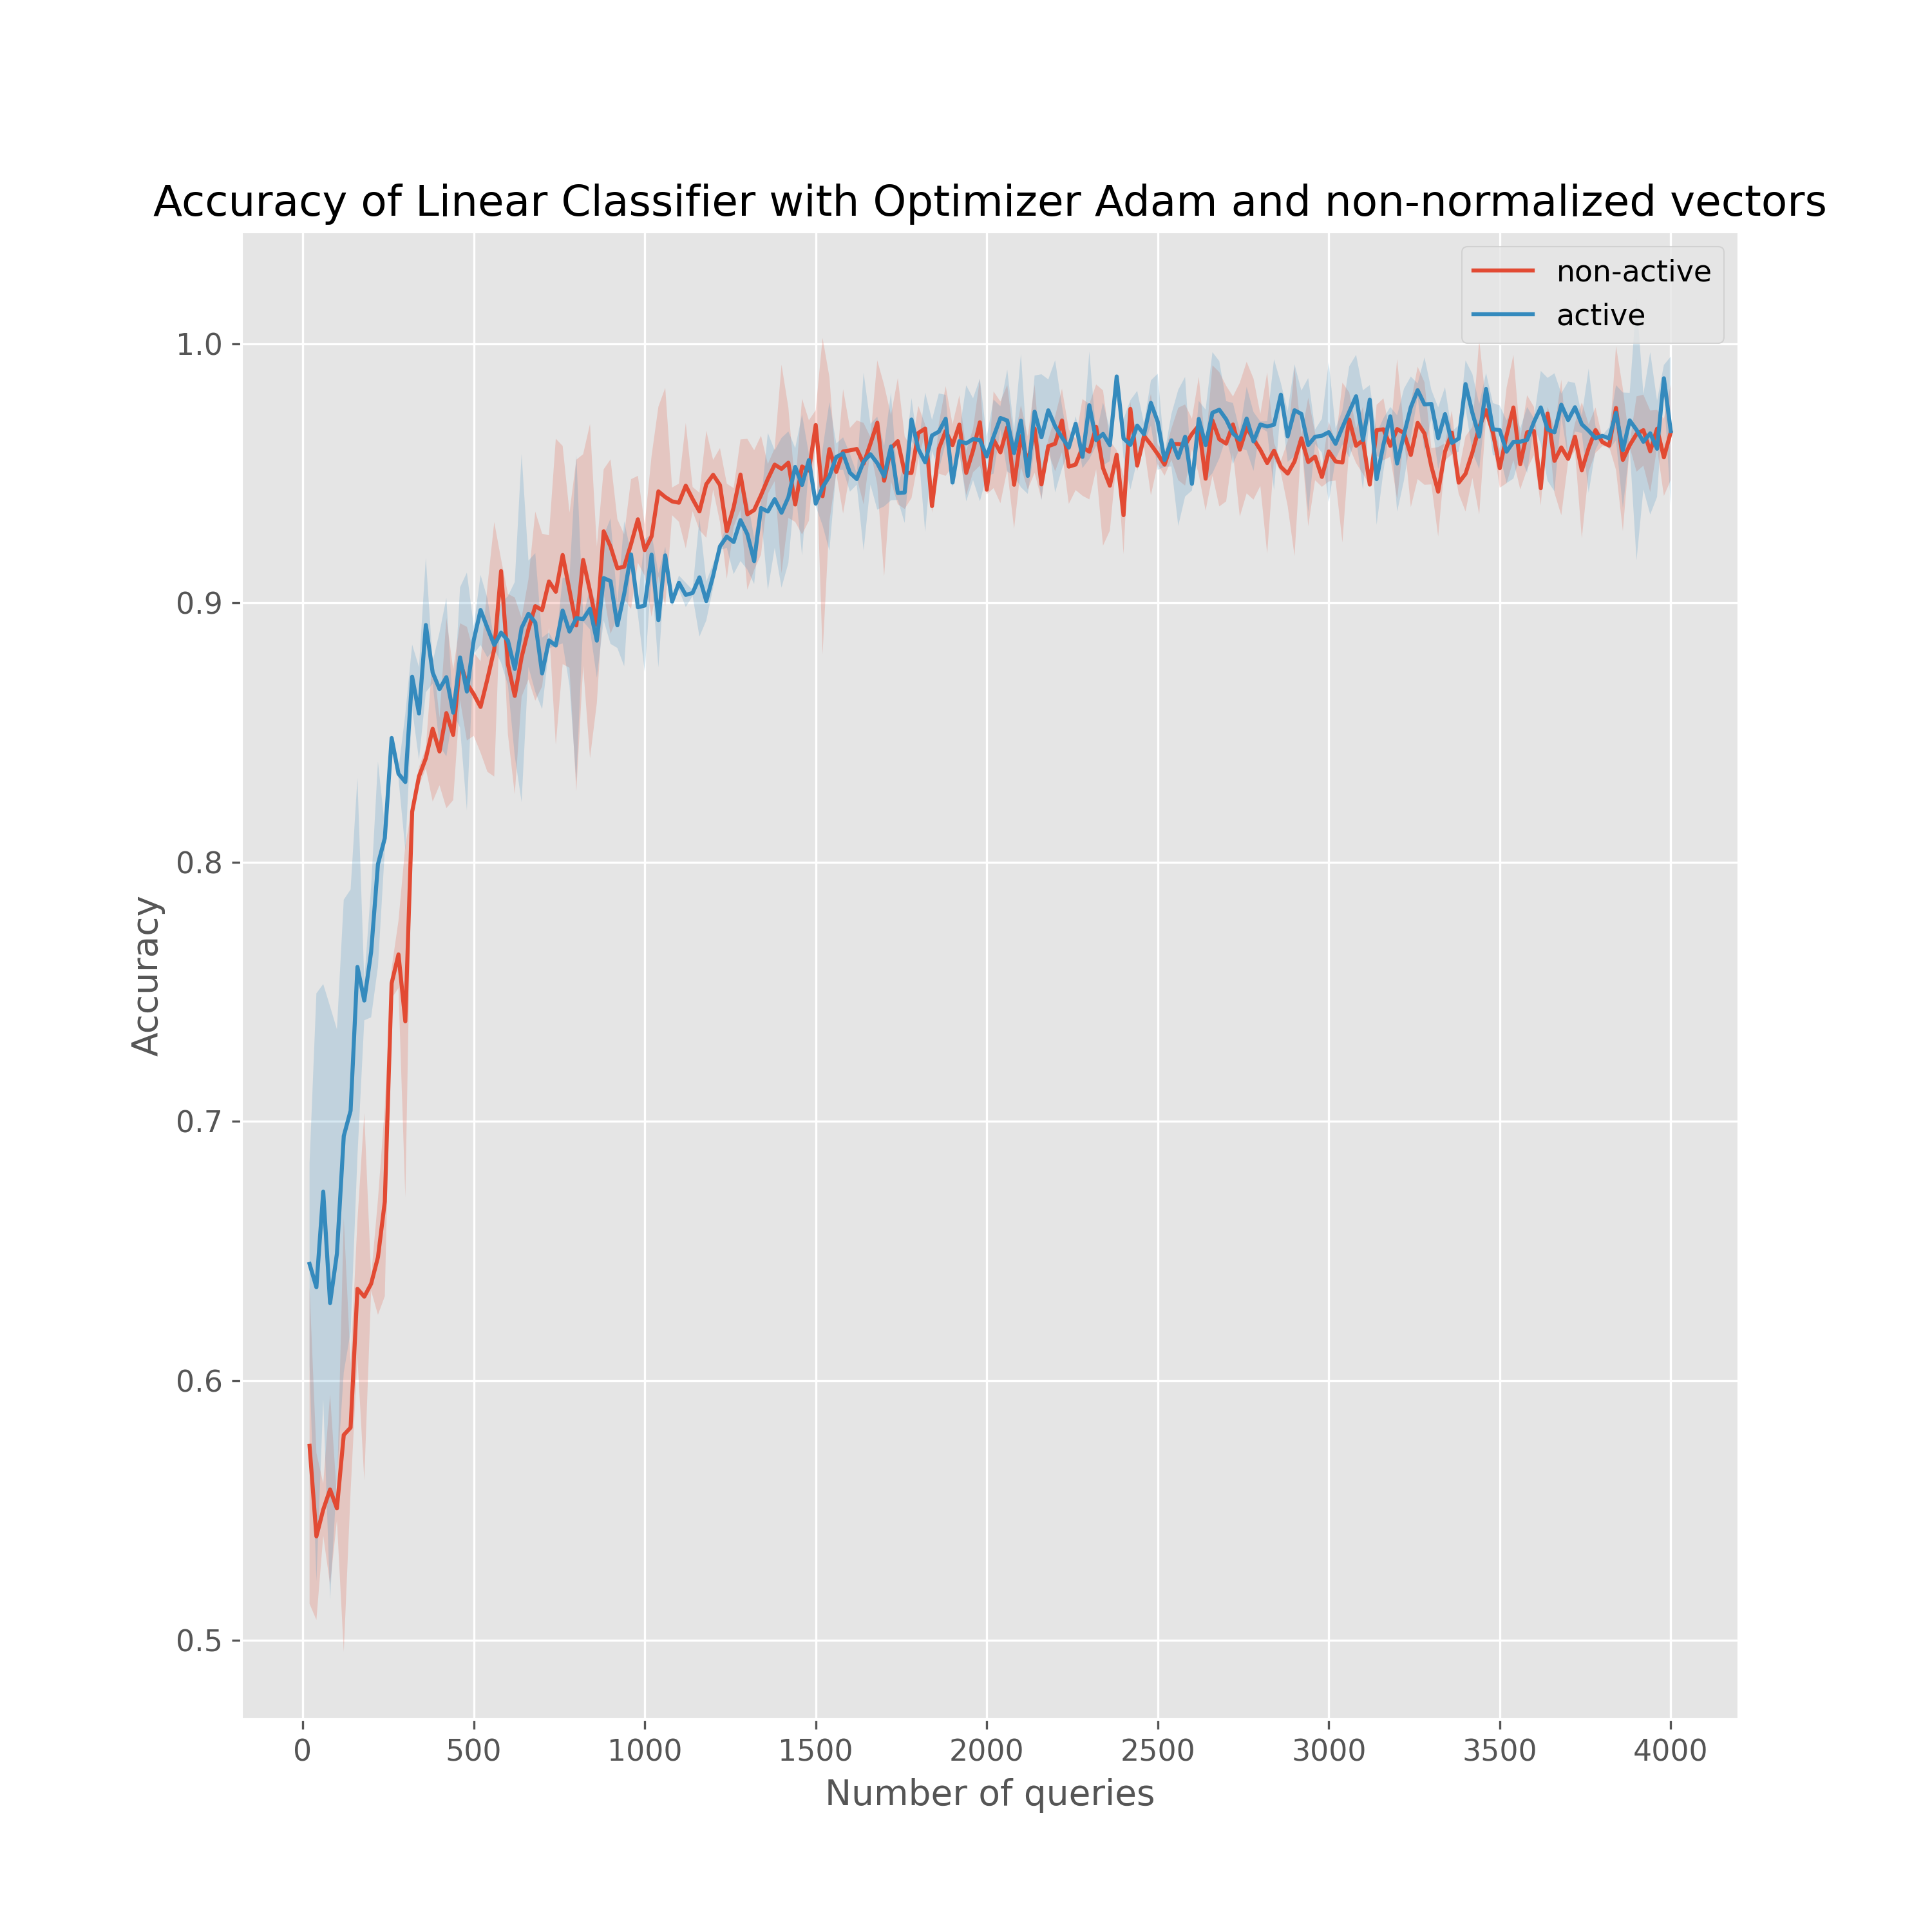
\includegraphics[width=\linewidth]{active-vs-base-moons-linear-loss-Adam-non-normalized-ci}
  \end{minipage}
  \caption{Performance SVM on non-normalized learned features Adam vs SGD}\label{fig:svm-non-normalized-ci}
\end{figure}

% add figures
\begin{figure}[!h]
  \centering
  \begin{minipage}{.45\textwidth}
    \centering
    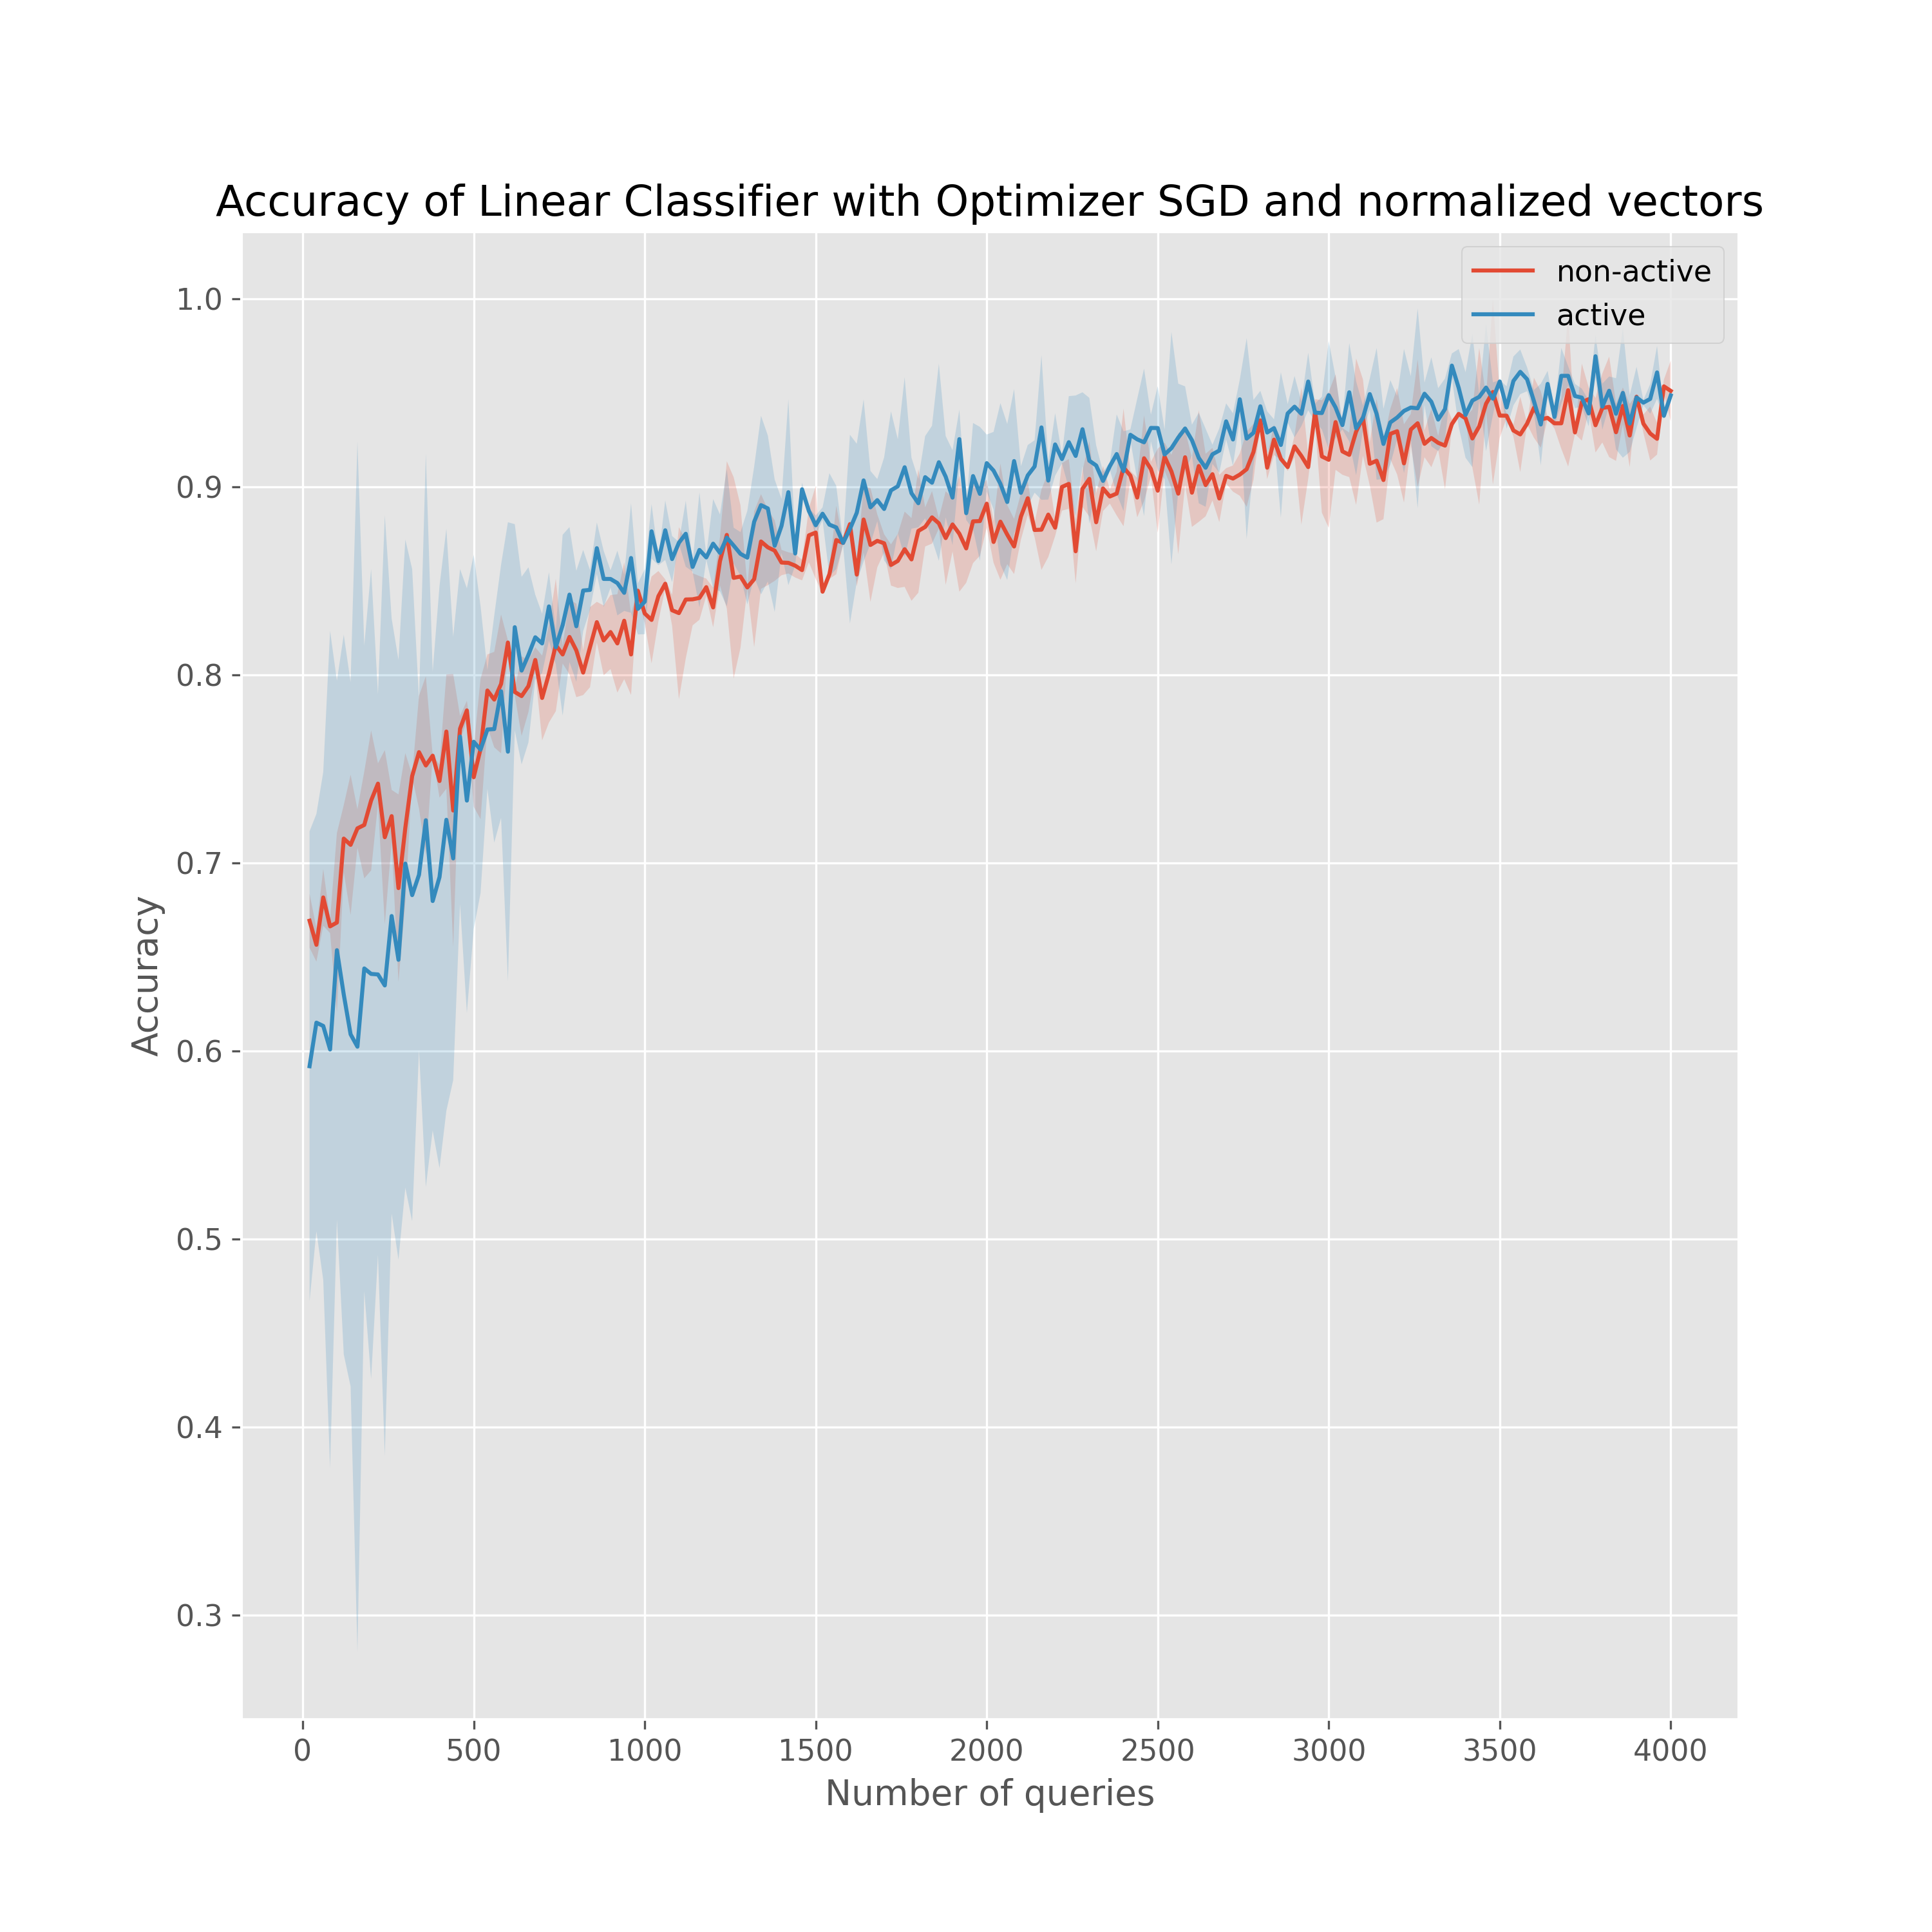
\includegraphics[width=\linewidth]{active-vs-base-moons-linear-loss-SGD-normalized-ci}
  \end{minipage}%
  \begin{minipage}{.45\textwidth}
    \centering
    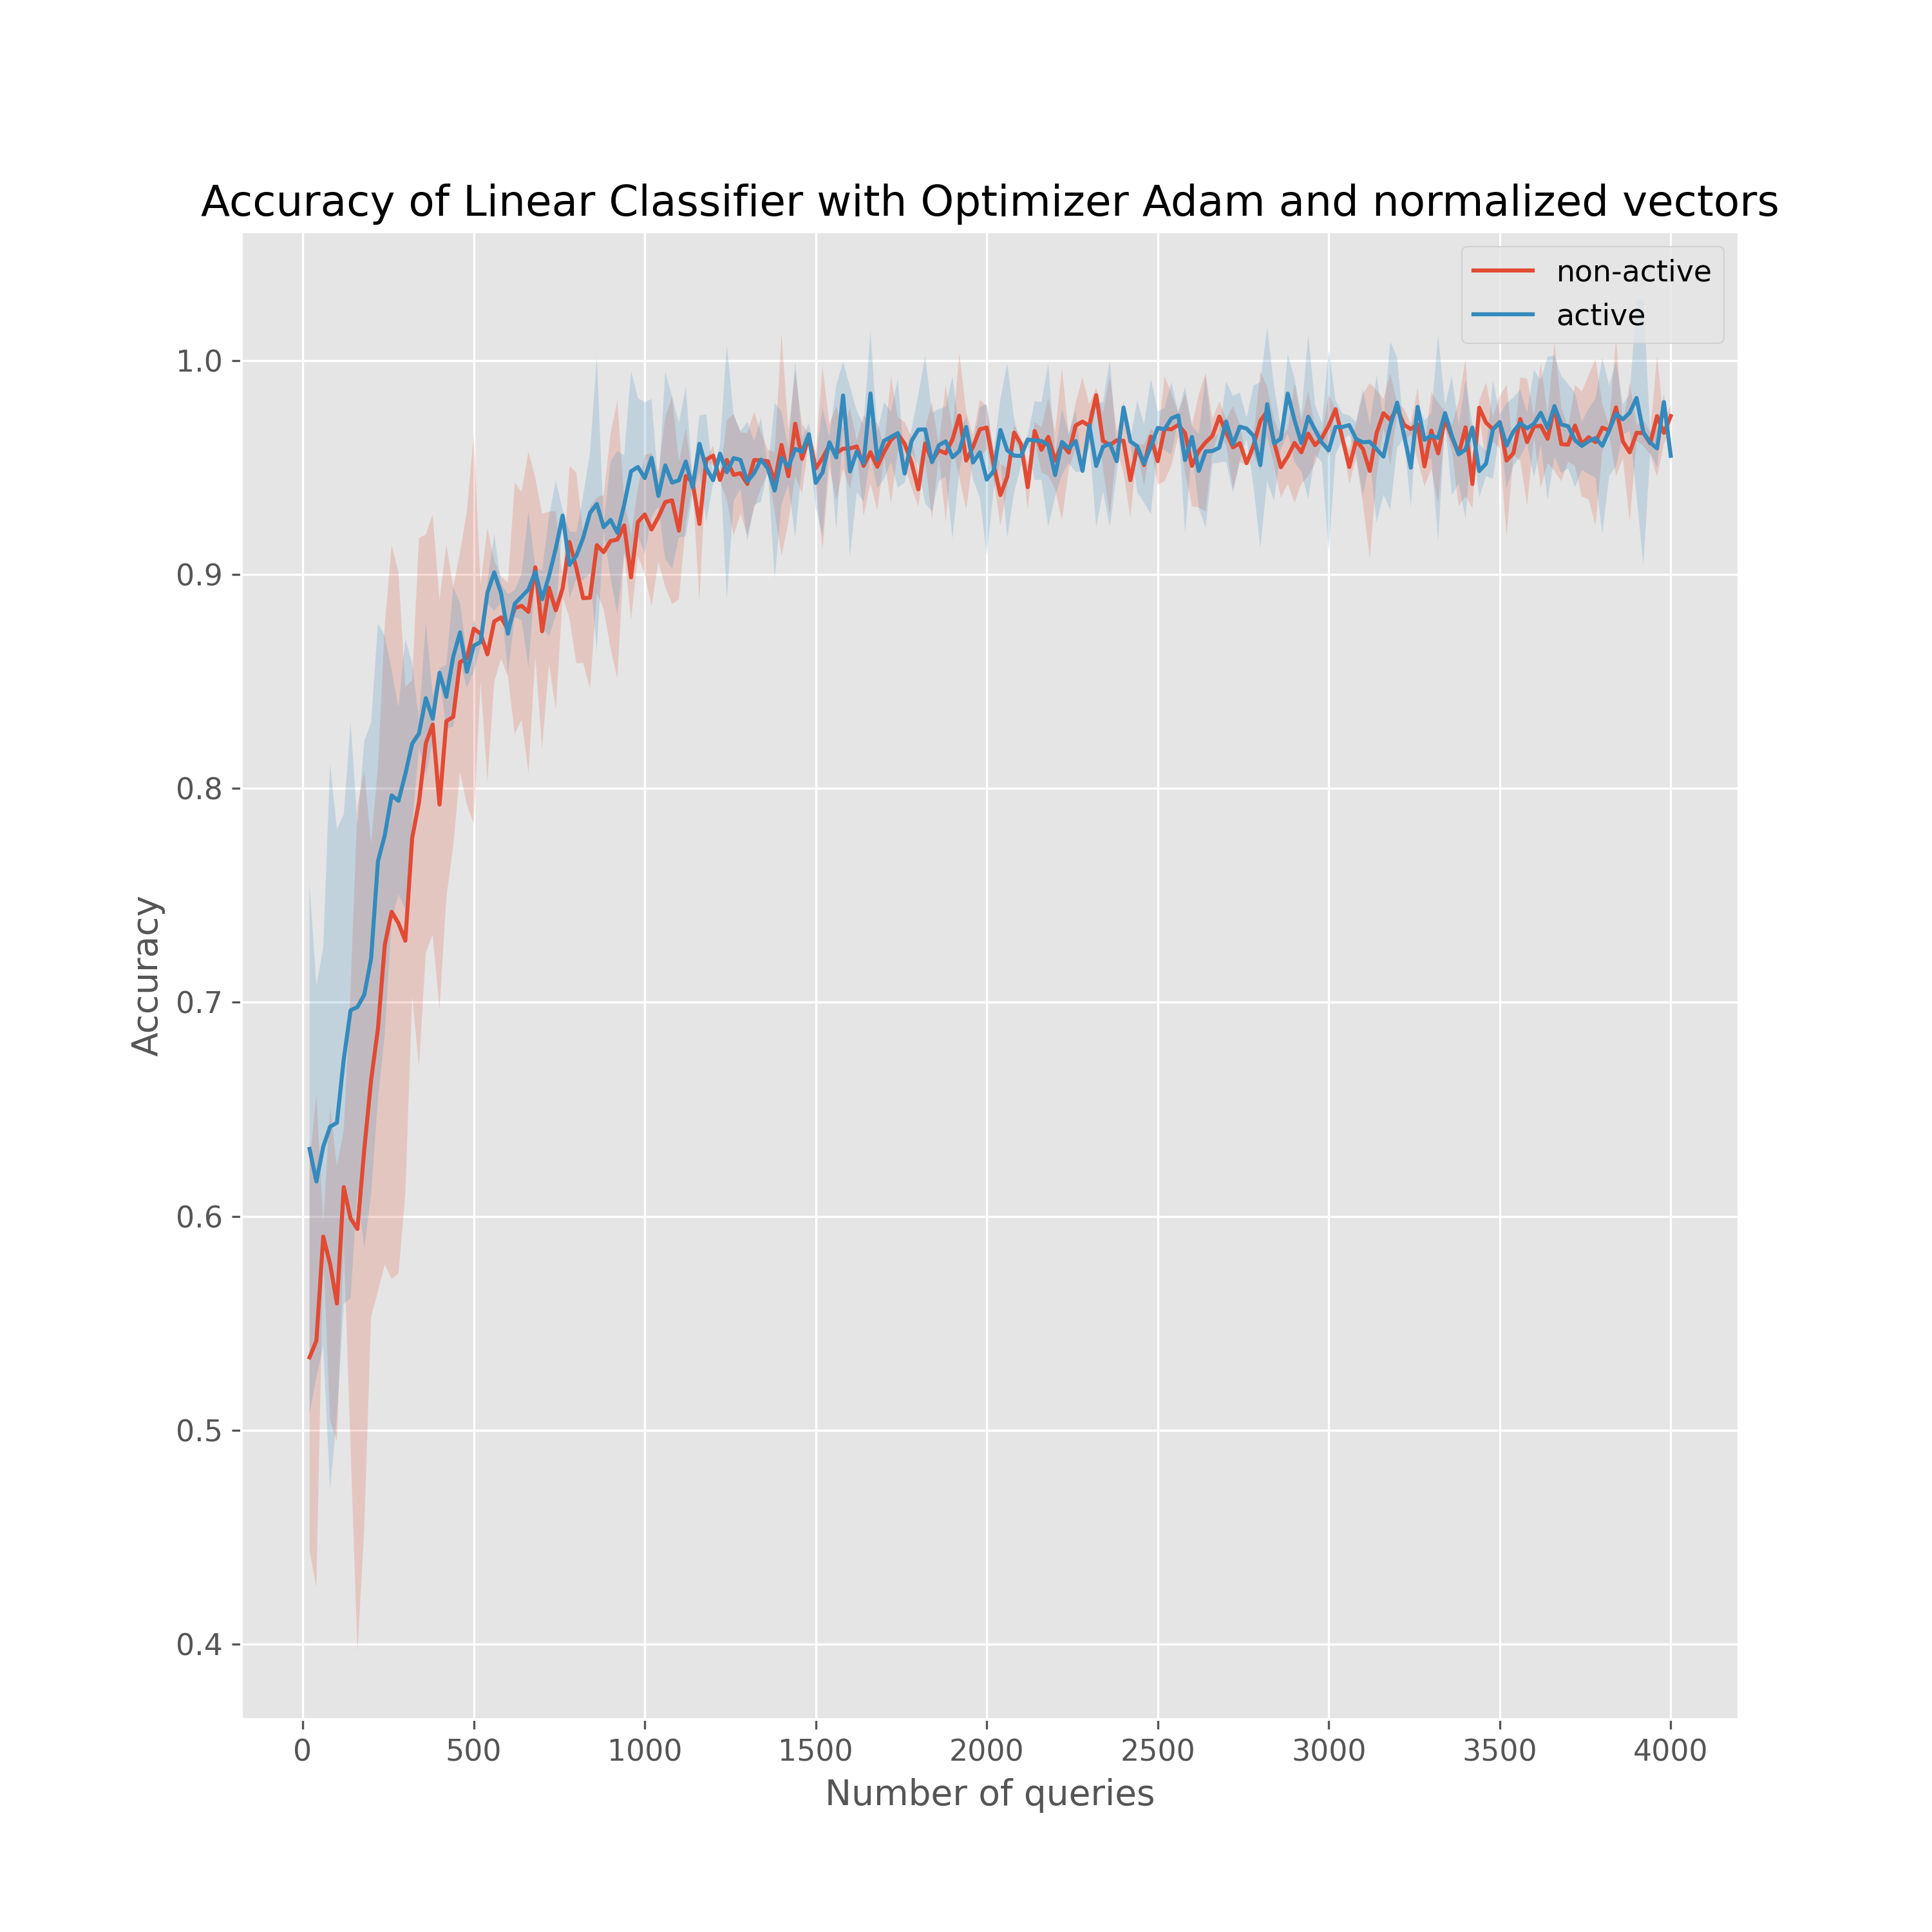
\includegraphics[width=\linewidth]{active-vs-base-moons-linear-loss-Adam-normalized-ci}
  \end{minipage}
  \caption{Performance SVM on normalized learned features Adam vs SGD}\label{fig:svm-normalized-ci}
\end{figure}

\subsection{Experiment 2: Comparison of L2 loss through time}
Using the exact setup as in Experiment 1, we report the results of the L2 loss through time for Active-NeuralUCB.
\begin{figure}[!h]
  \centering
  \begin{minipage}{.45\textwidth}
    \centering
    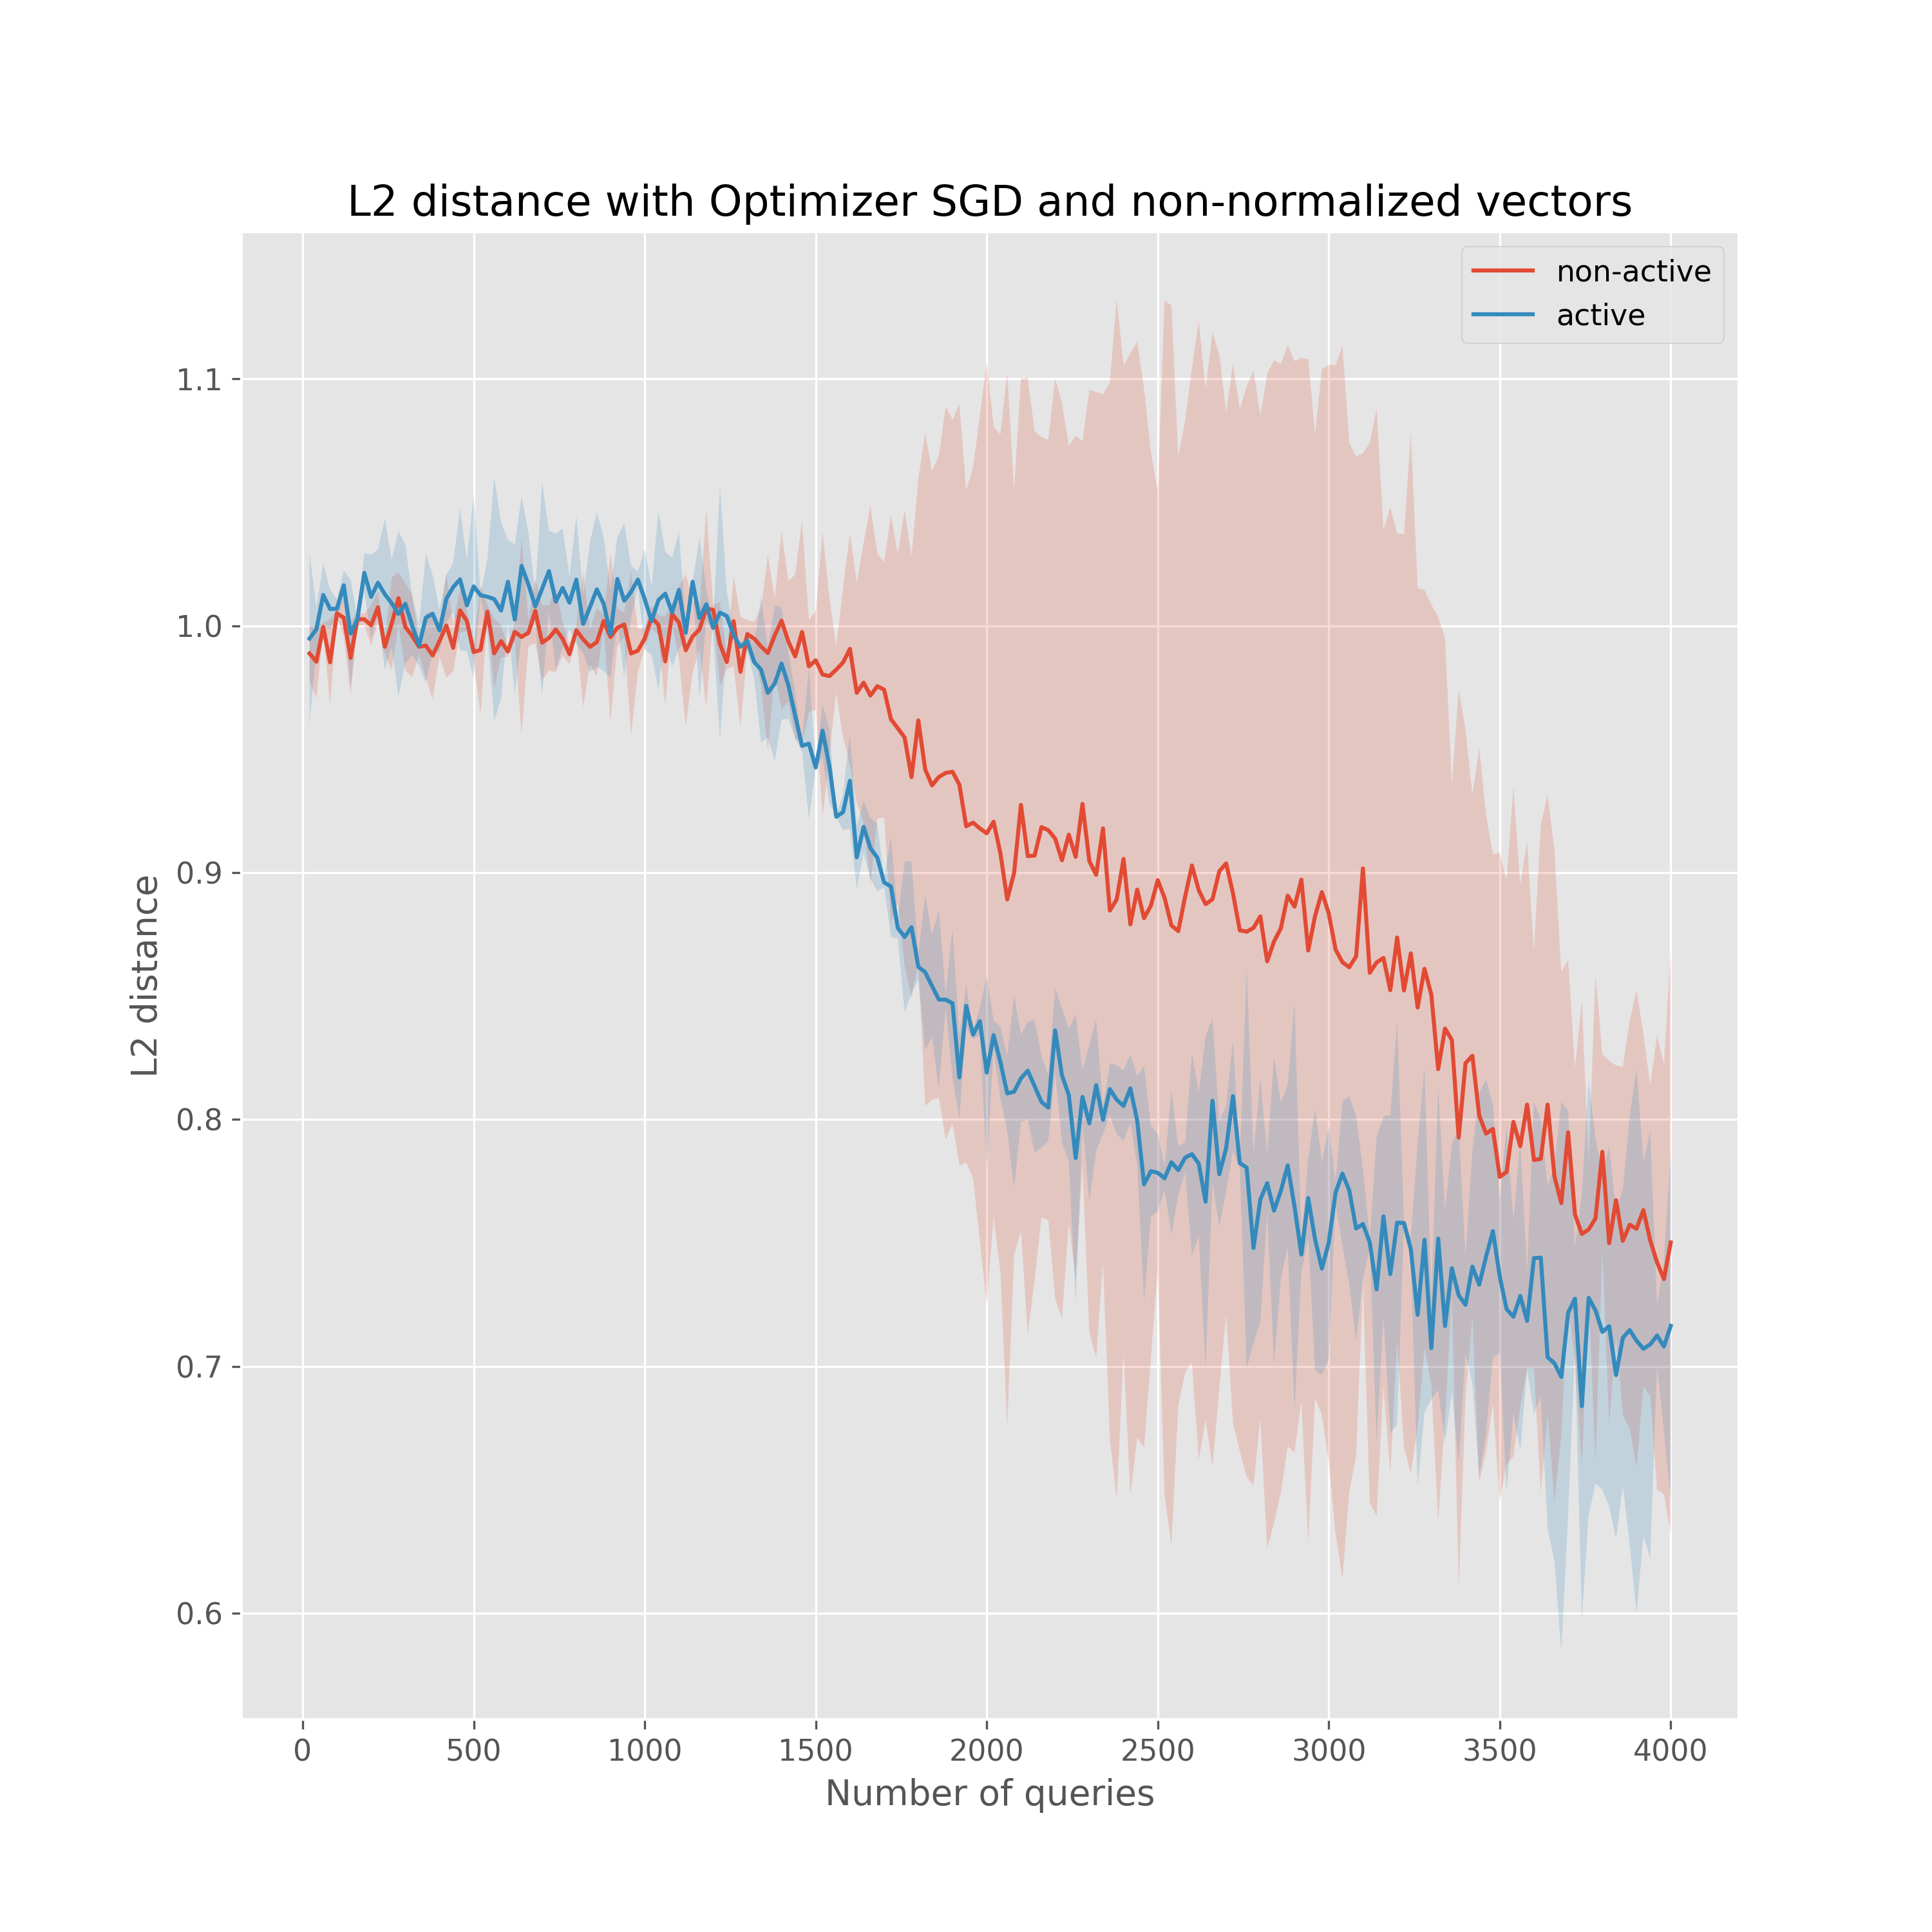
\includegraphics[width=\linewidth]{active-vs-base-moons-l2-loss-SGD-non-normalized-ci}
  \end{minipage}%
  \begin{minipage}{.45\textwidth}
    \centering
    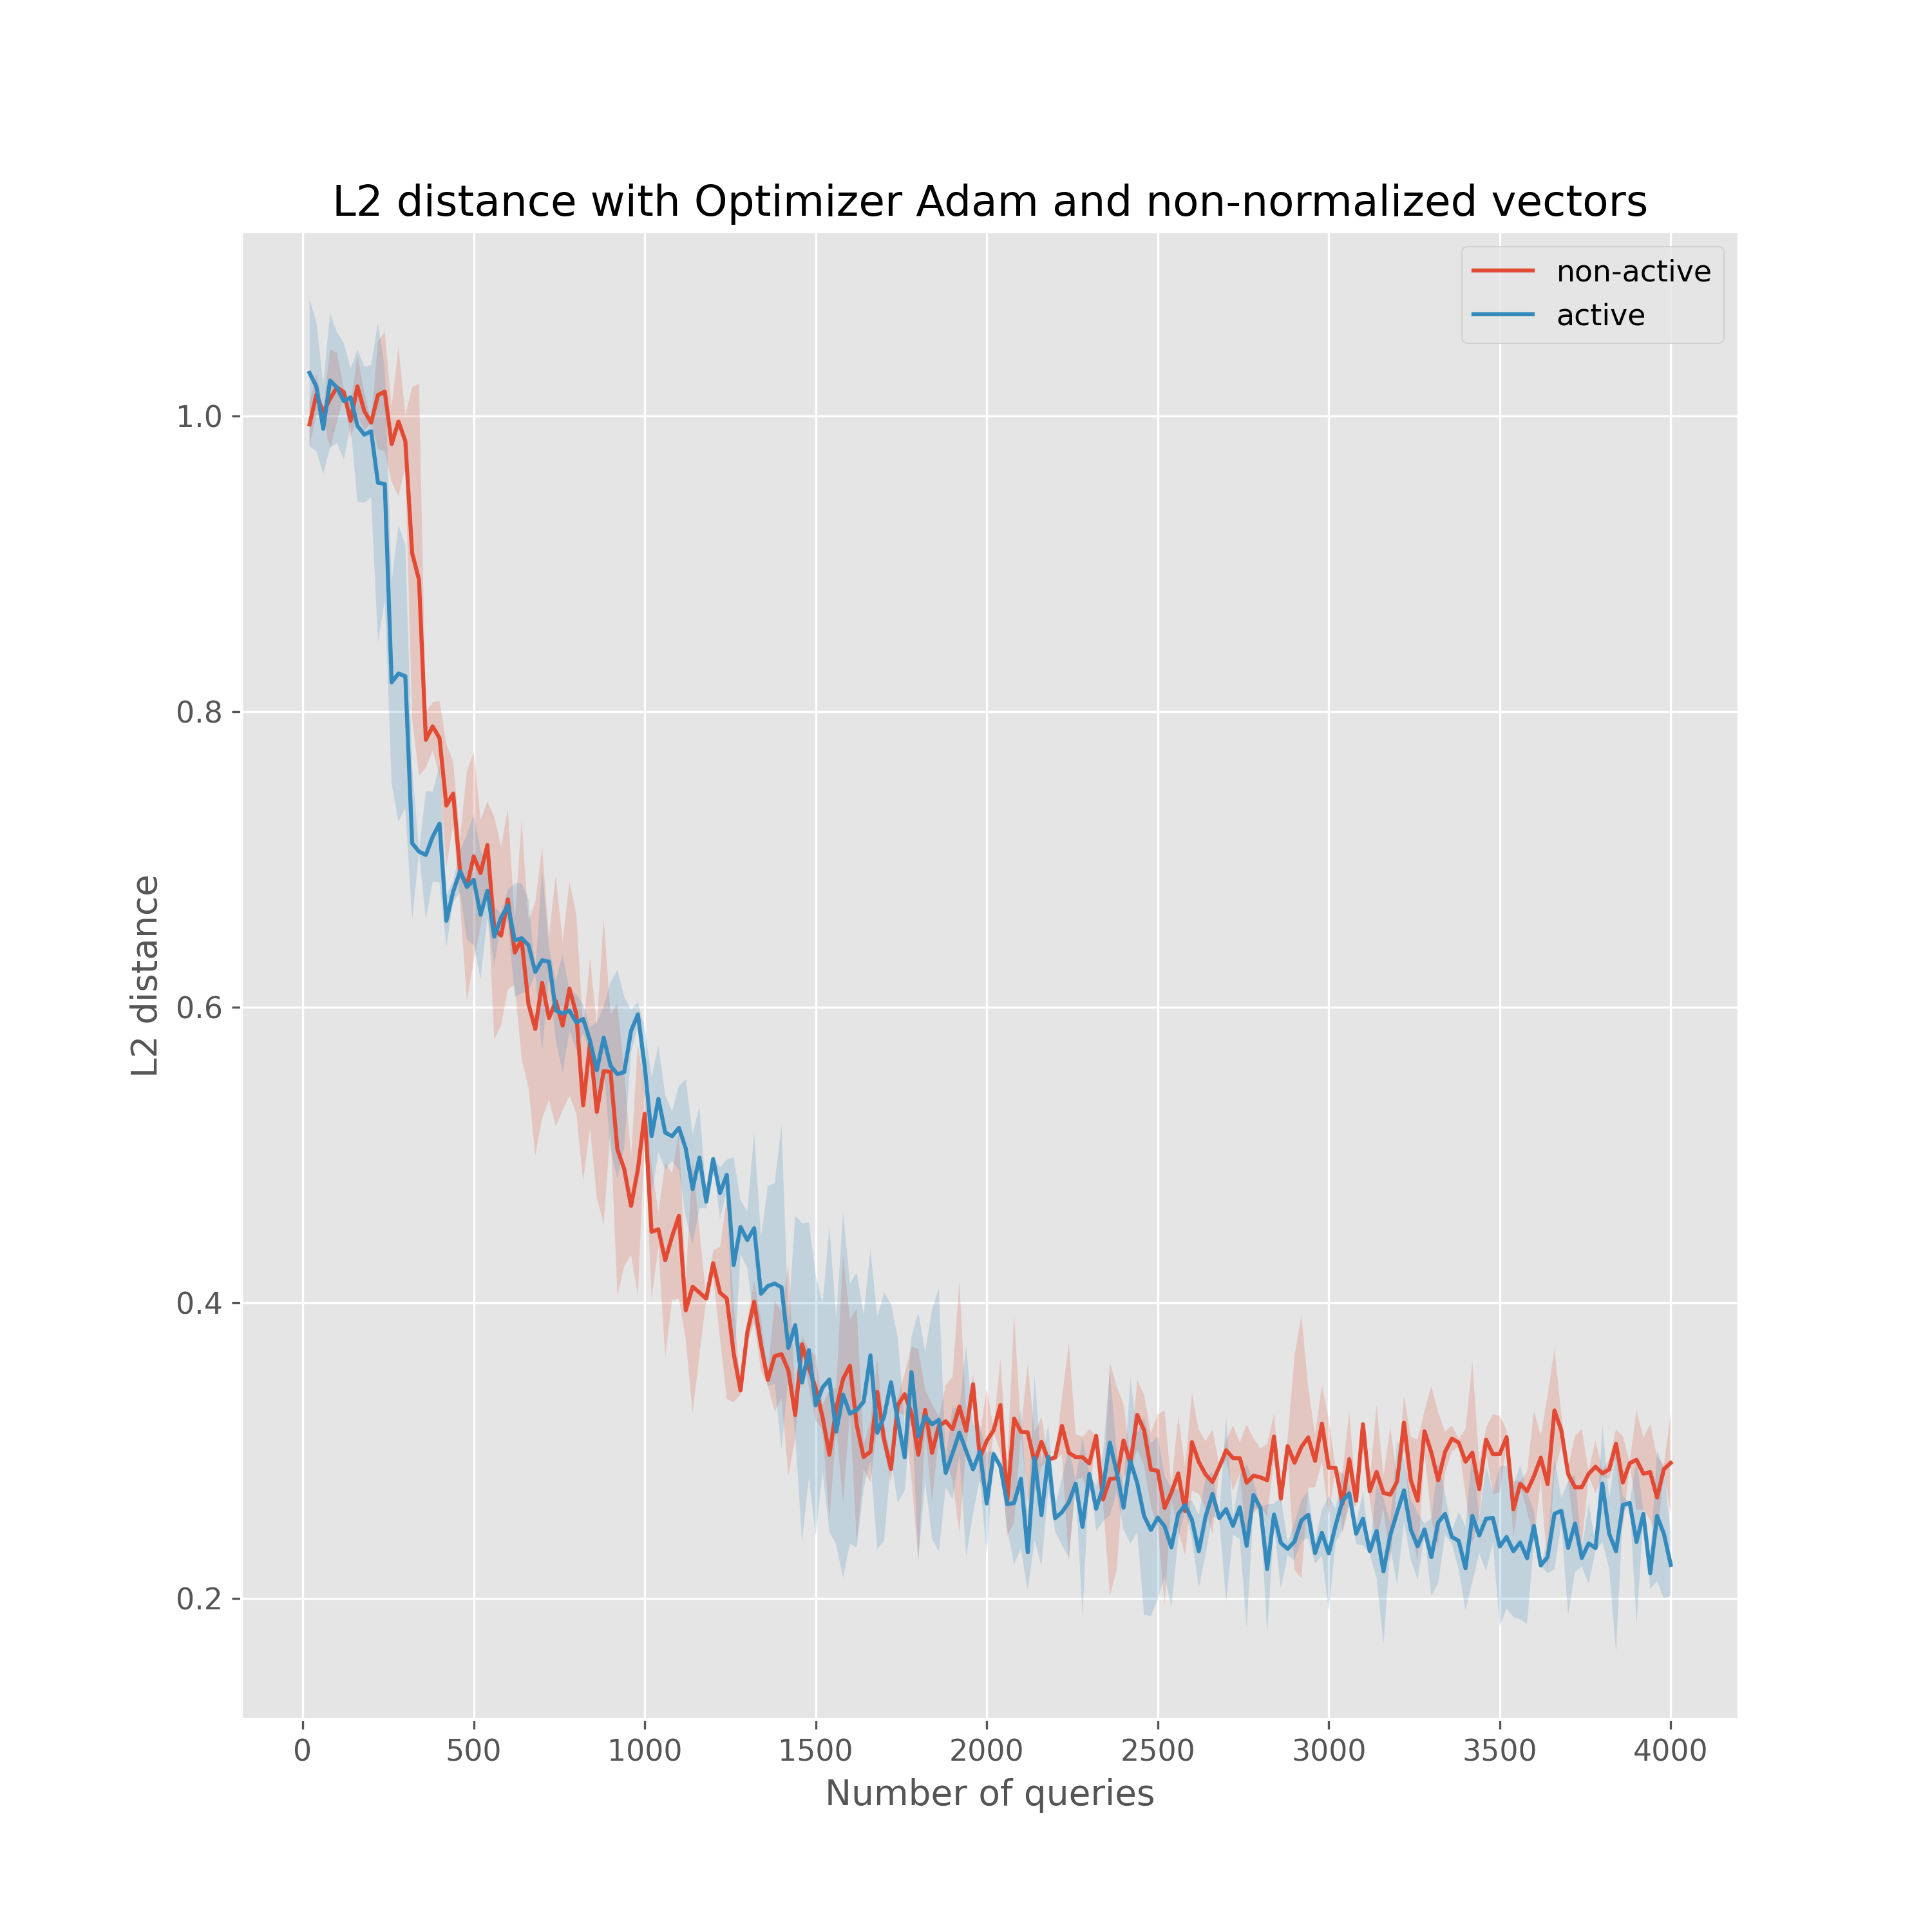
\includegraphics[width=\linewidth]{active-vs-base-moons-l2-loss-Adam-non-normalized-ci}
  \end{minipage}
  \caption{Performance SVM on non-normalized learned features Adam vs SGD}\label{fig:l2-loss-non-normalized-ci}
\end{figure}

% add figures
\begin{figure}[!h]
  \centering
  \begin{minipage}{.45\textwidth}
    \centering
    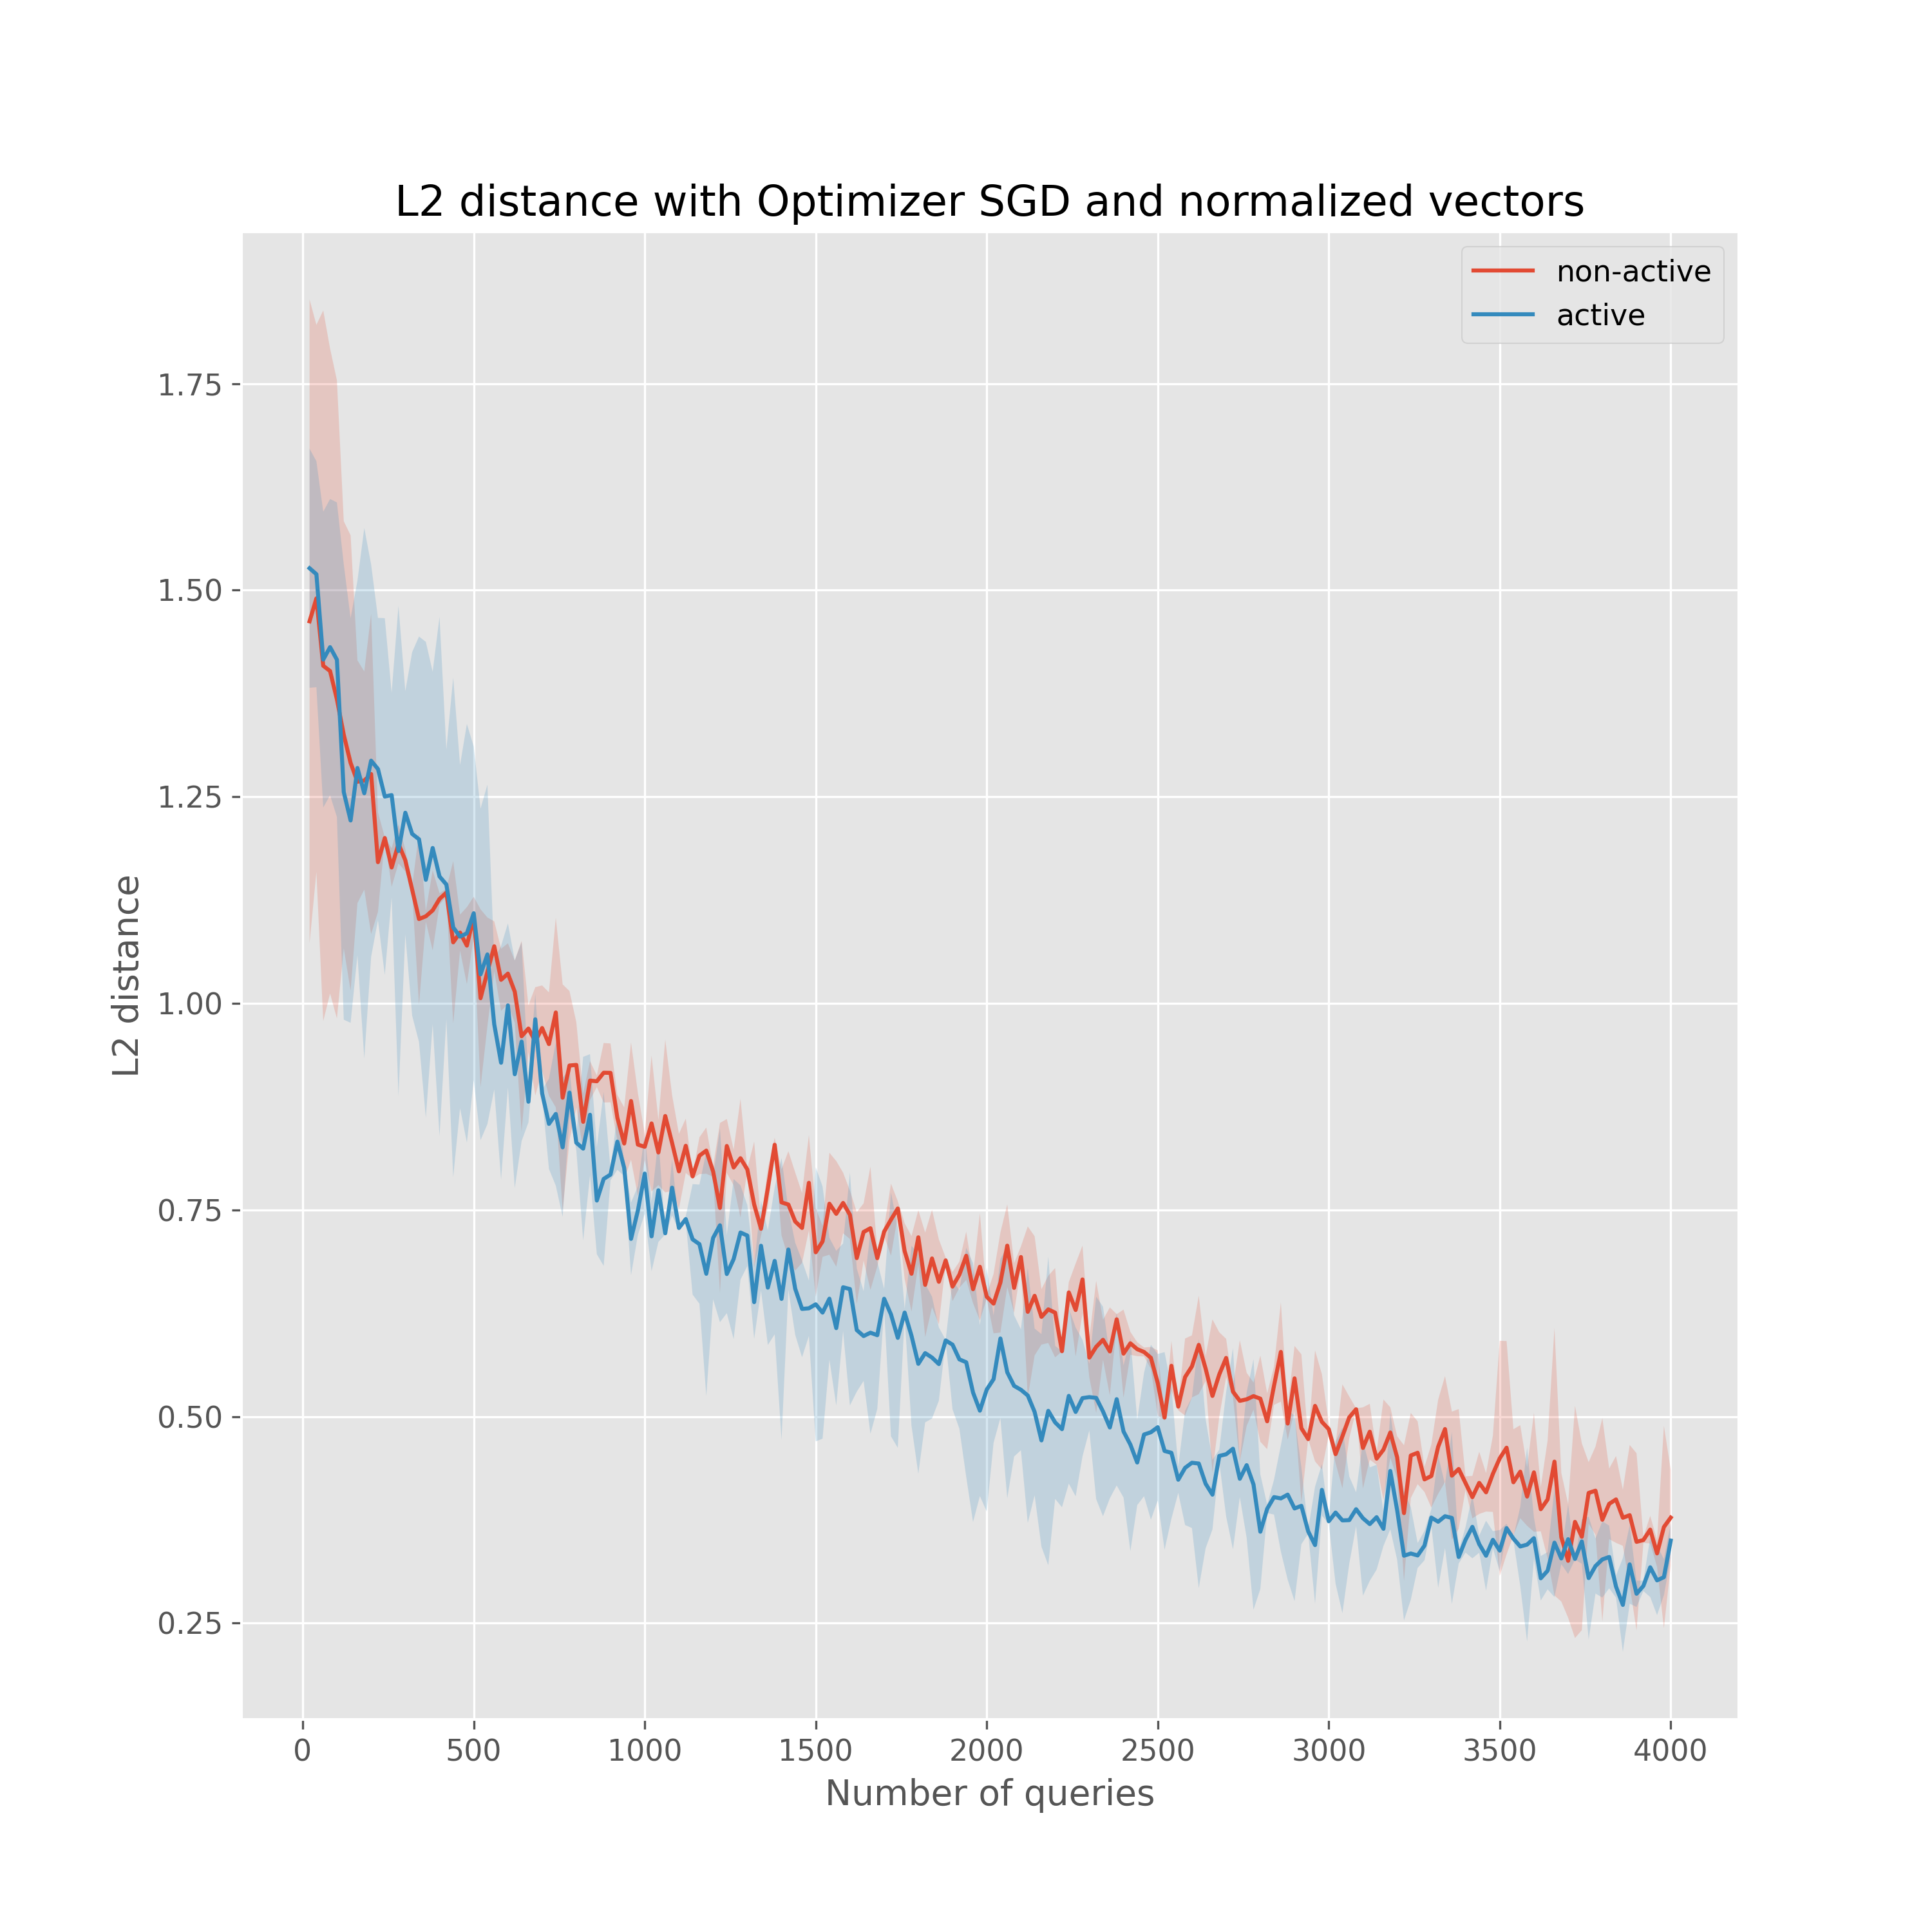
\includegraphics[width=\linewidth]{active-vs-base-moons-l2-loss-SGD-normalized-ci}
  \end{minipage}%
  \begin{minipage}{.45\textwidth}
    \centering
    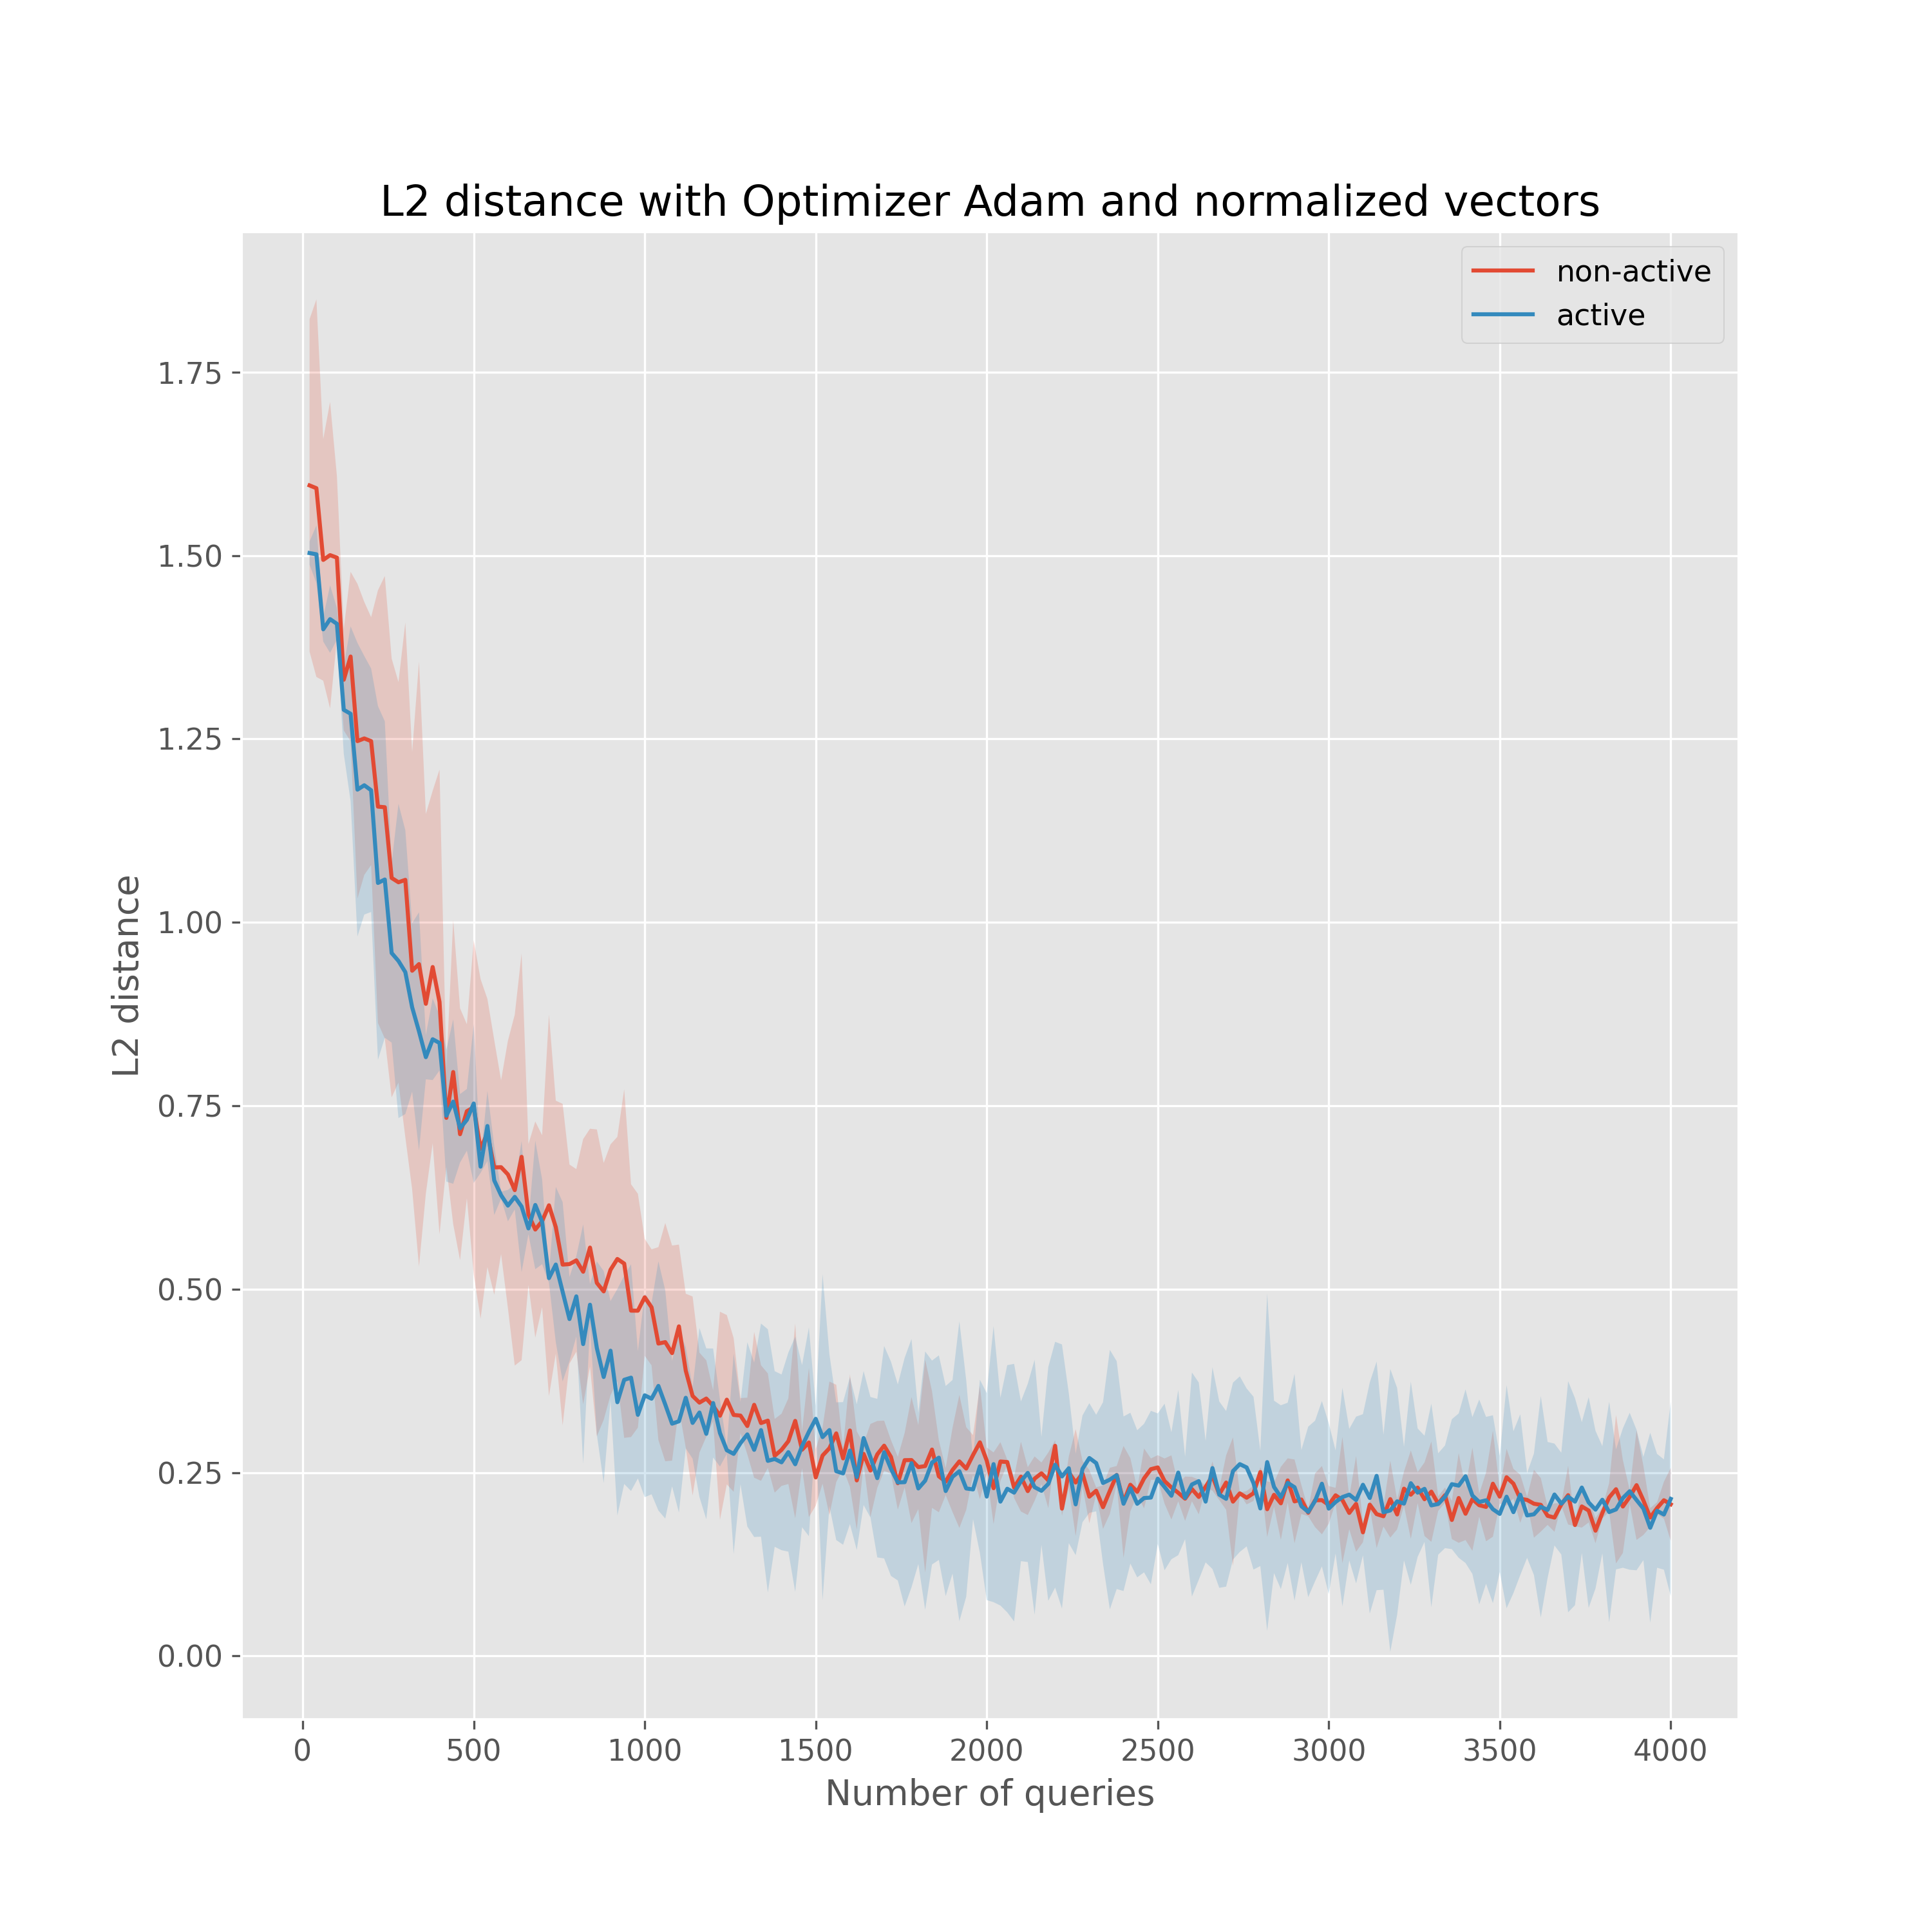
\includegraphics[width=\linewidth]{active-vs-base-moons-l2-loss-Adam-normalized-ci}
  \end{minipage}
  \caption{Performance SVM on normalized learned features Adam vs SGD}\label{fig:l2-loss-normalized-ci}
\end{figure}

\subsection{Experiment 3: Regret of OnSim-NeuralUCB}
We observe the performance of OnSim-NeuralUCB by compring the regret of the algorithm with the regret of an epsilon-greedy
neural network with the same architecture and hyperparameters. We report the results only Adam with normalized and unormalized versions
Like in the previous experiment all graphs contain thegit mean and a 95\% confidence interval. We also compare various values for
the exploration parameter.\footnote{The appendix contains a more thorough graph with even more values.}


\subsection{LinearUCB}
\subparagraph{Dataset:}
To test the linear version of our algorithm we created a blobs dataset.
Every point is drawn from the following process. Assume that $x_i' \sim \mathcal{N}((0, 0)^\top,I_2)$ and $p_i \sim \text{Bernoulli}(p)$ where $p$ is
some parameter.
Then the data point $x_i$ is drawn from the follwing process
\[x_i = \begin{bmatrix} 3 & 0\\ 0 & 1\\ \end{bmatrix} x_i' -(1-p_i)
\begin{bmatrix}
1\\
1\\
\end{bmatrix}
+ p_i
\begin{bmatrix}
1\\
0\\
\end{bmatrix}
\]
which corresponds to two blobs one placed on the left axis and one on the right axis.
We say that two points are similar if they share the same value of $p$.
We refer to this dataset as the Blobs dataset.

\begin{algorithm}
  \setstretch{1.2}
    \SetKwInOut{Input}{Input}
    \Input{Rounds $T$ and exploration parameter $\alpha$}
    $A \gets I_{n^2}$\;
    $b \gets 0_{n^2}$\;
    \For{$t \in [T]$}{
      $\theta_t \gets A^{-1}b$
      Observe $K$ pairs of vectors $x^k \in R^n$, $y^k \in R^n$\;
      Create $z_{t,k} = (x_1^ky_1^k, x_1^ky_1^k, \dots, x_n^k y_{n-1}^k, x_n^k y_n^k)$\;
      \For{$k \in [K]$}{
        $p_{t,a} \gets  \alpha \sqrt{z_{t,k} A^{-1} x_{t,a}}$
        \label{change:active-linucb}
      }
      Choose action pair $k_t = \text{argmax}_ap_{t,a}$ with ties broken arbitrarily.\;
      Observe label $ r_t \in \{-1,1 \}$\;
      $A \gets A + z_{t,k_t}z_{t,k_t}^\top$\;
      $b \gets z_{t,j_t}r_t$\;
    }
    \caption{Active-LinUCB}\label{algo:active-linucb}
\end{algorithm}


\subsubsection{Experiment 1: Effectiveness of active learning balanced and unbalanced datset}
We test the effectiveness of active learning on the balanced and unbalanced datasets.
For the unbalanced instance we use $p = 0.1$ but provide the results of an l2 loss assuming that the real distribution of the data is balanced.
This is done to simulate a situation in which our collected unlabeled data is based and to show the improvement in robustness of the
algorithm. The plots contain the mean and the 95\% confidence interval for the regret over 30 runs of each algorithm.

\begin{figure}[!h]
  \centering
  \begin{minipage}{.45\textwidth}
    \centering
    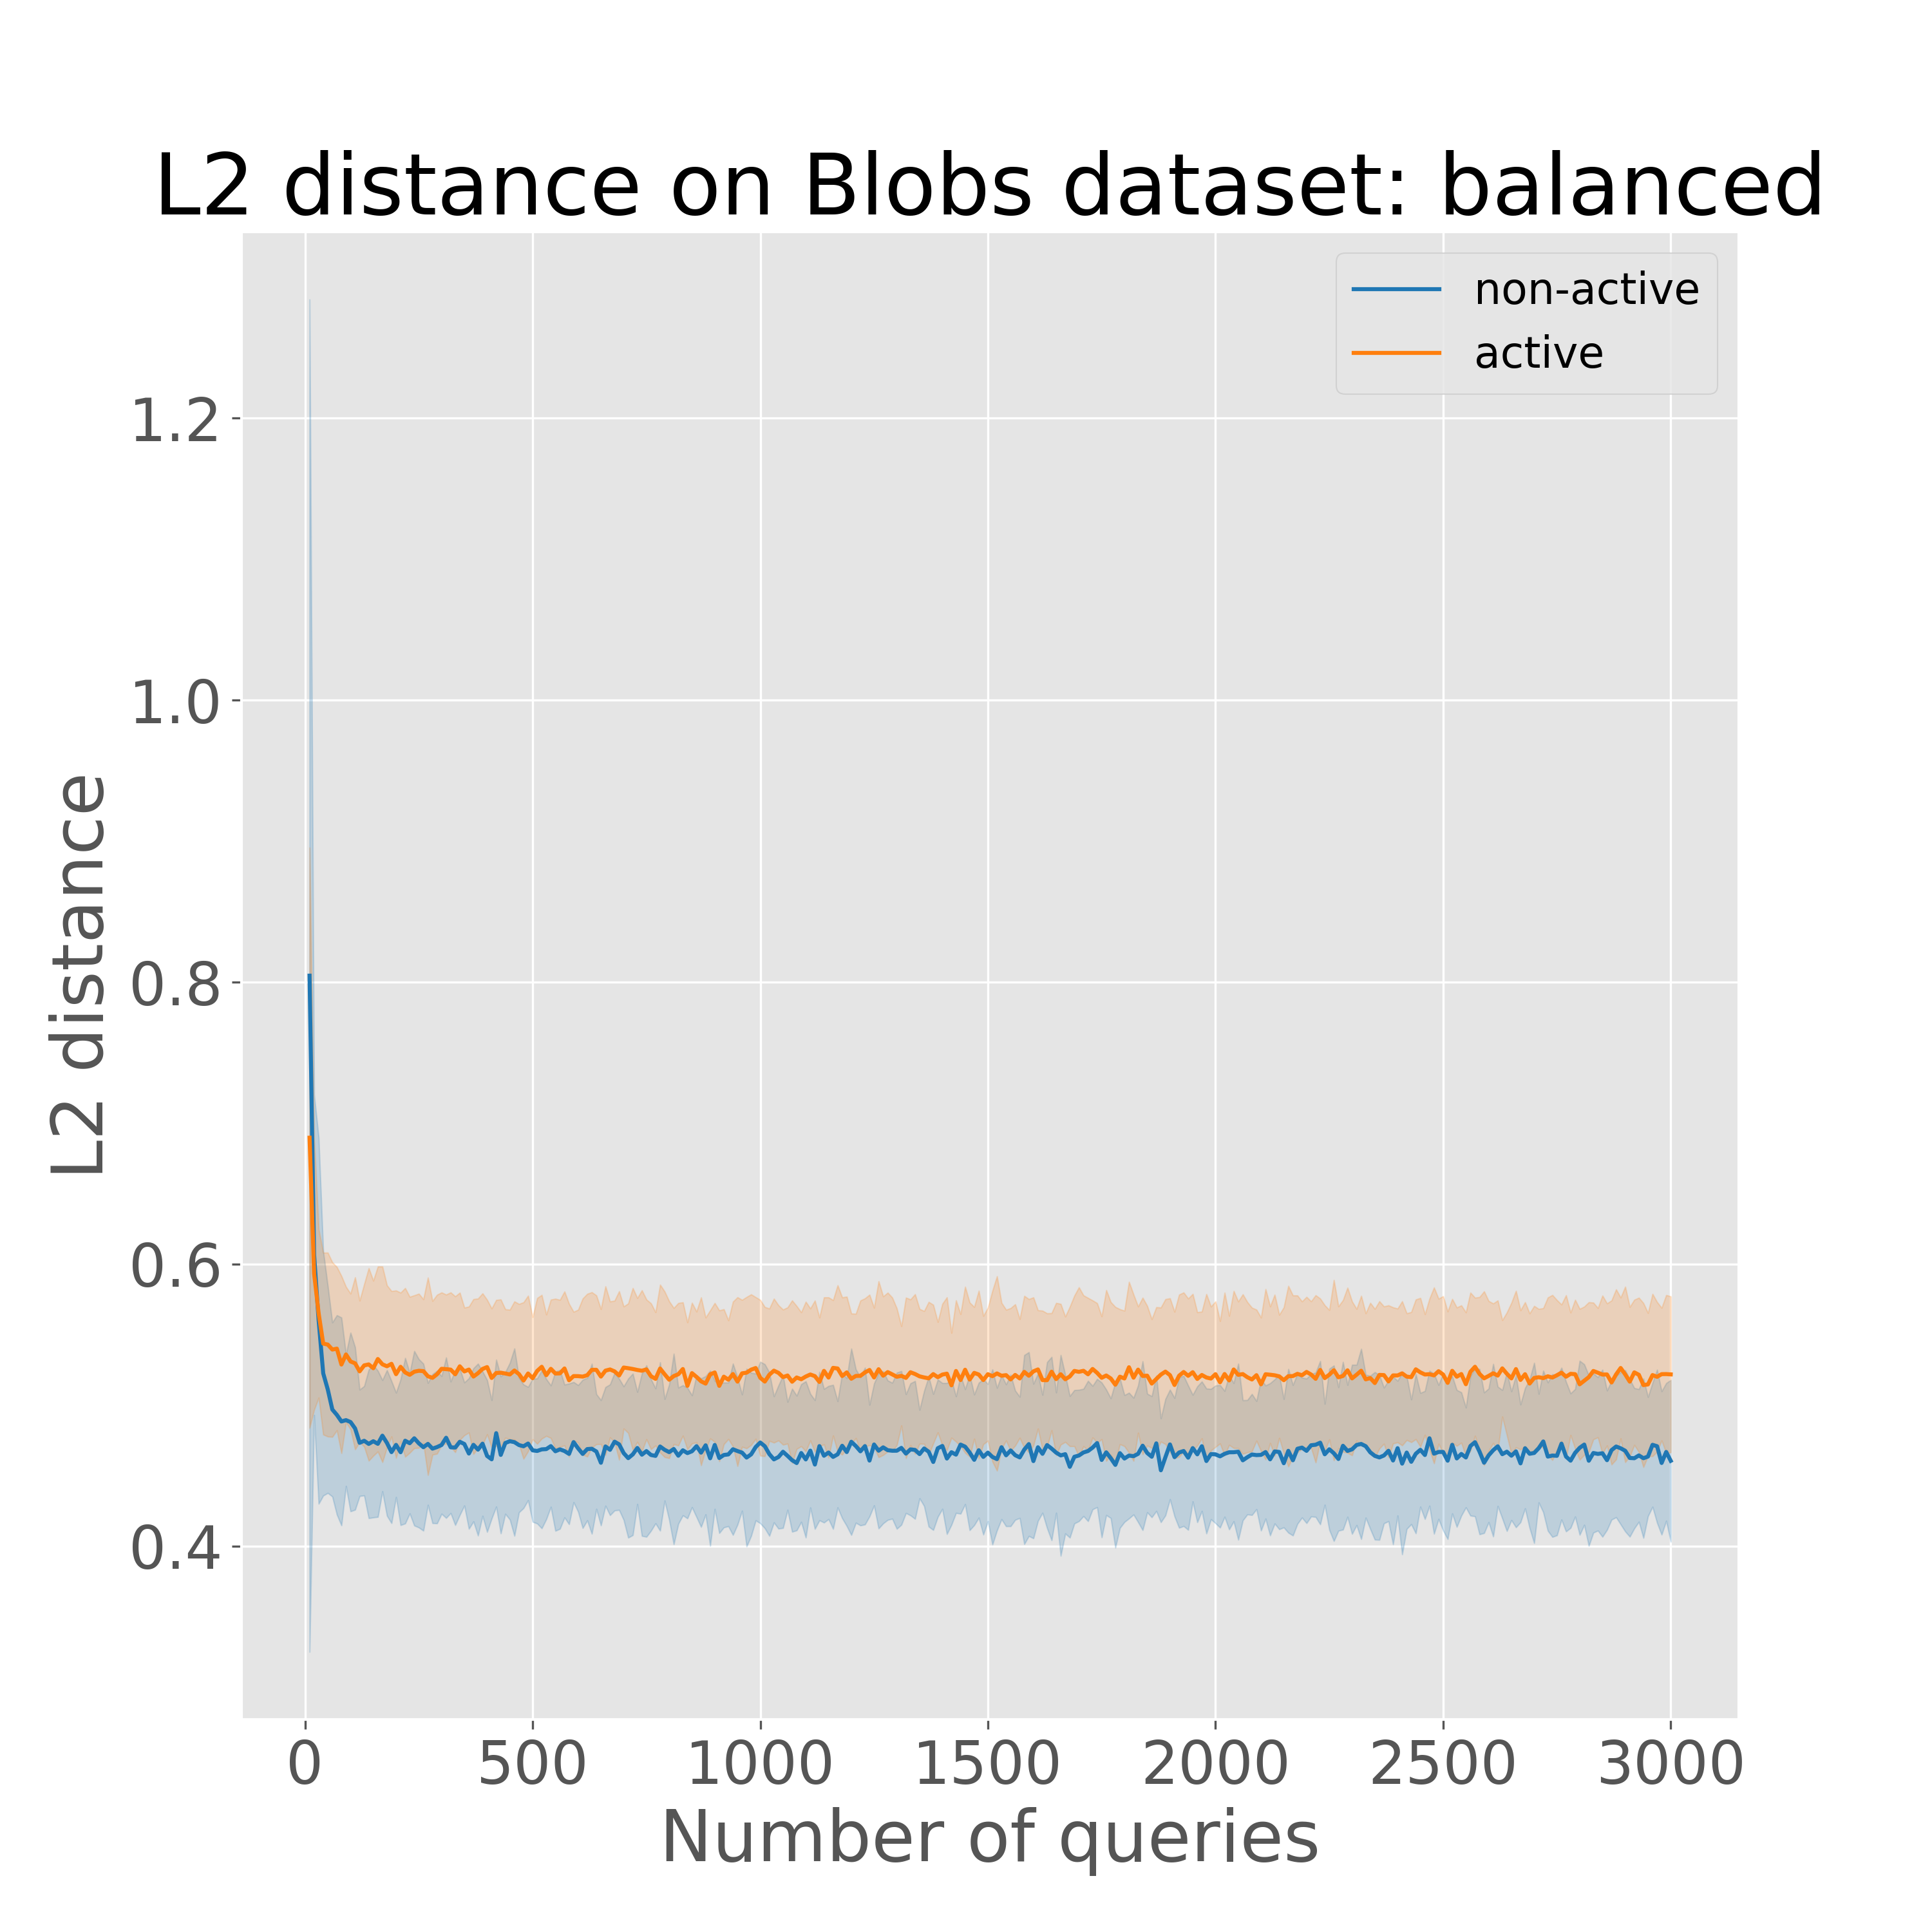
\includegraphics[width=\linewidth]{active-vs-base-blobs-l2-loss_balanced-ci}
    \caption{Active vs non-active balanced datasets}\label{fig:linucb-blobs-regret-no-regime-change}
  \end{minipage}%
  \begin{minipage}{.45\textwidth}
    \centering
    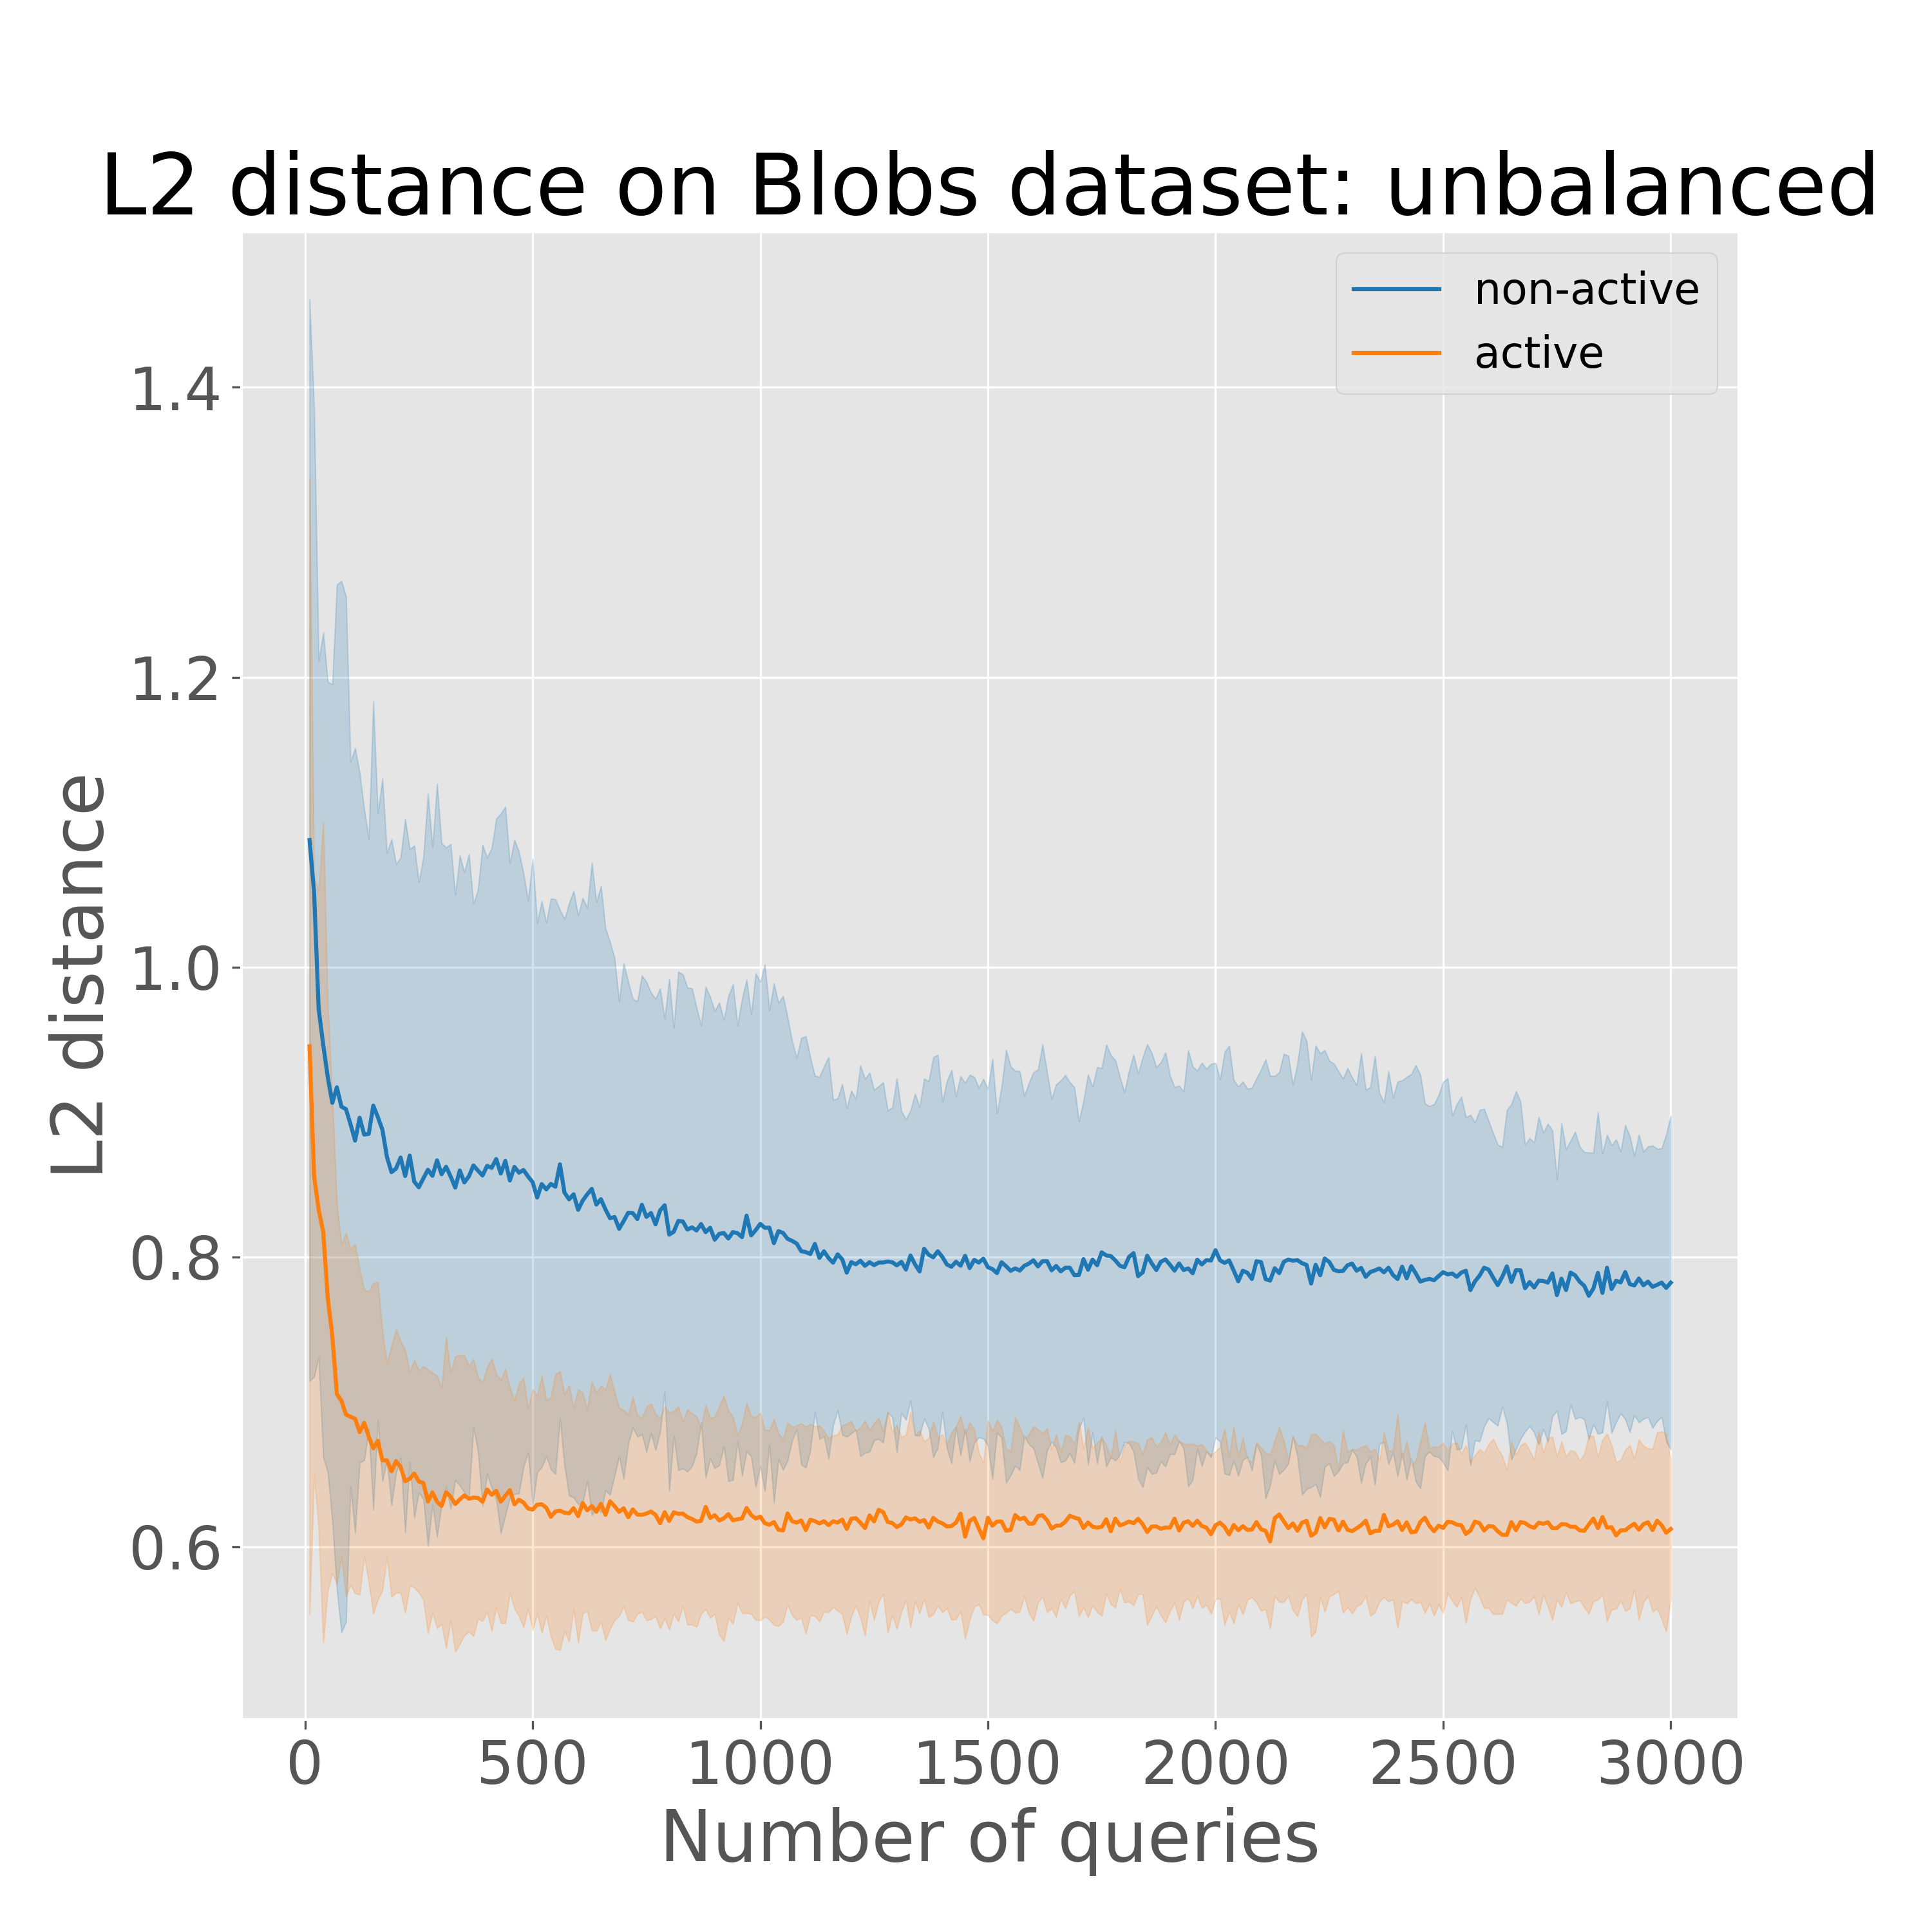
\includegraphics[width=\linewidth]{active-vs-base-blobs-l2-loss_unbalanced-ci}
    \caption{Active vs non active balanced datasets}\label{fig:linucb-blobs-regret-regime-change}
  \end{minipage}
\end{figure}


\subsubsection{Experiment 2: Regret of active similarity with regime shifts}
To show that our approach leads to enhanced robustness we assume that we find ourselves in a situation
where the might be regime shifts in the data in the sense that the underlying distribution at which the data is provided
to the algorithm changes.

In particular, in the situation below we assume that initially the data is provided to us where there is an equal changce of getting a point
from the left blob and right blob but there at every time-step there is a $1/3000$ chance that
we will have a regime shift where the data is now sampled such that $p = 0.1$.
Plots (\ref{fig:linucb-blobs-regret-no-regime-change}) and (\ref{fig:linucb-blobs-regret-regime-change}) indicate the mean regret of the algorithm at the end
and the error bars depict the the $2.5$ and $97.5$ quantiles observed from 30 runs.

\begin{figure}[!h]
  \centering
  \begin{minipage}{.45\textwidth}
    \centering
    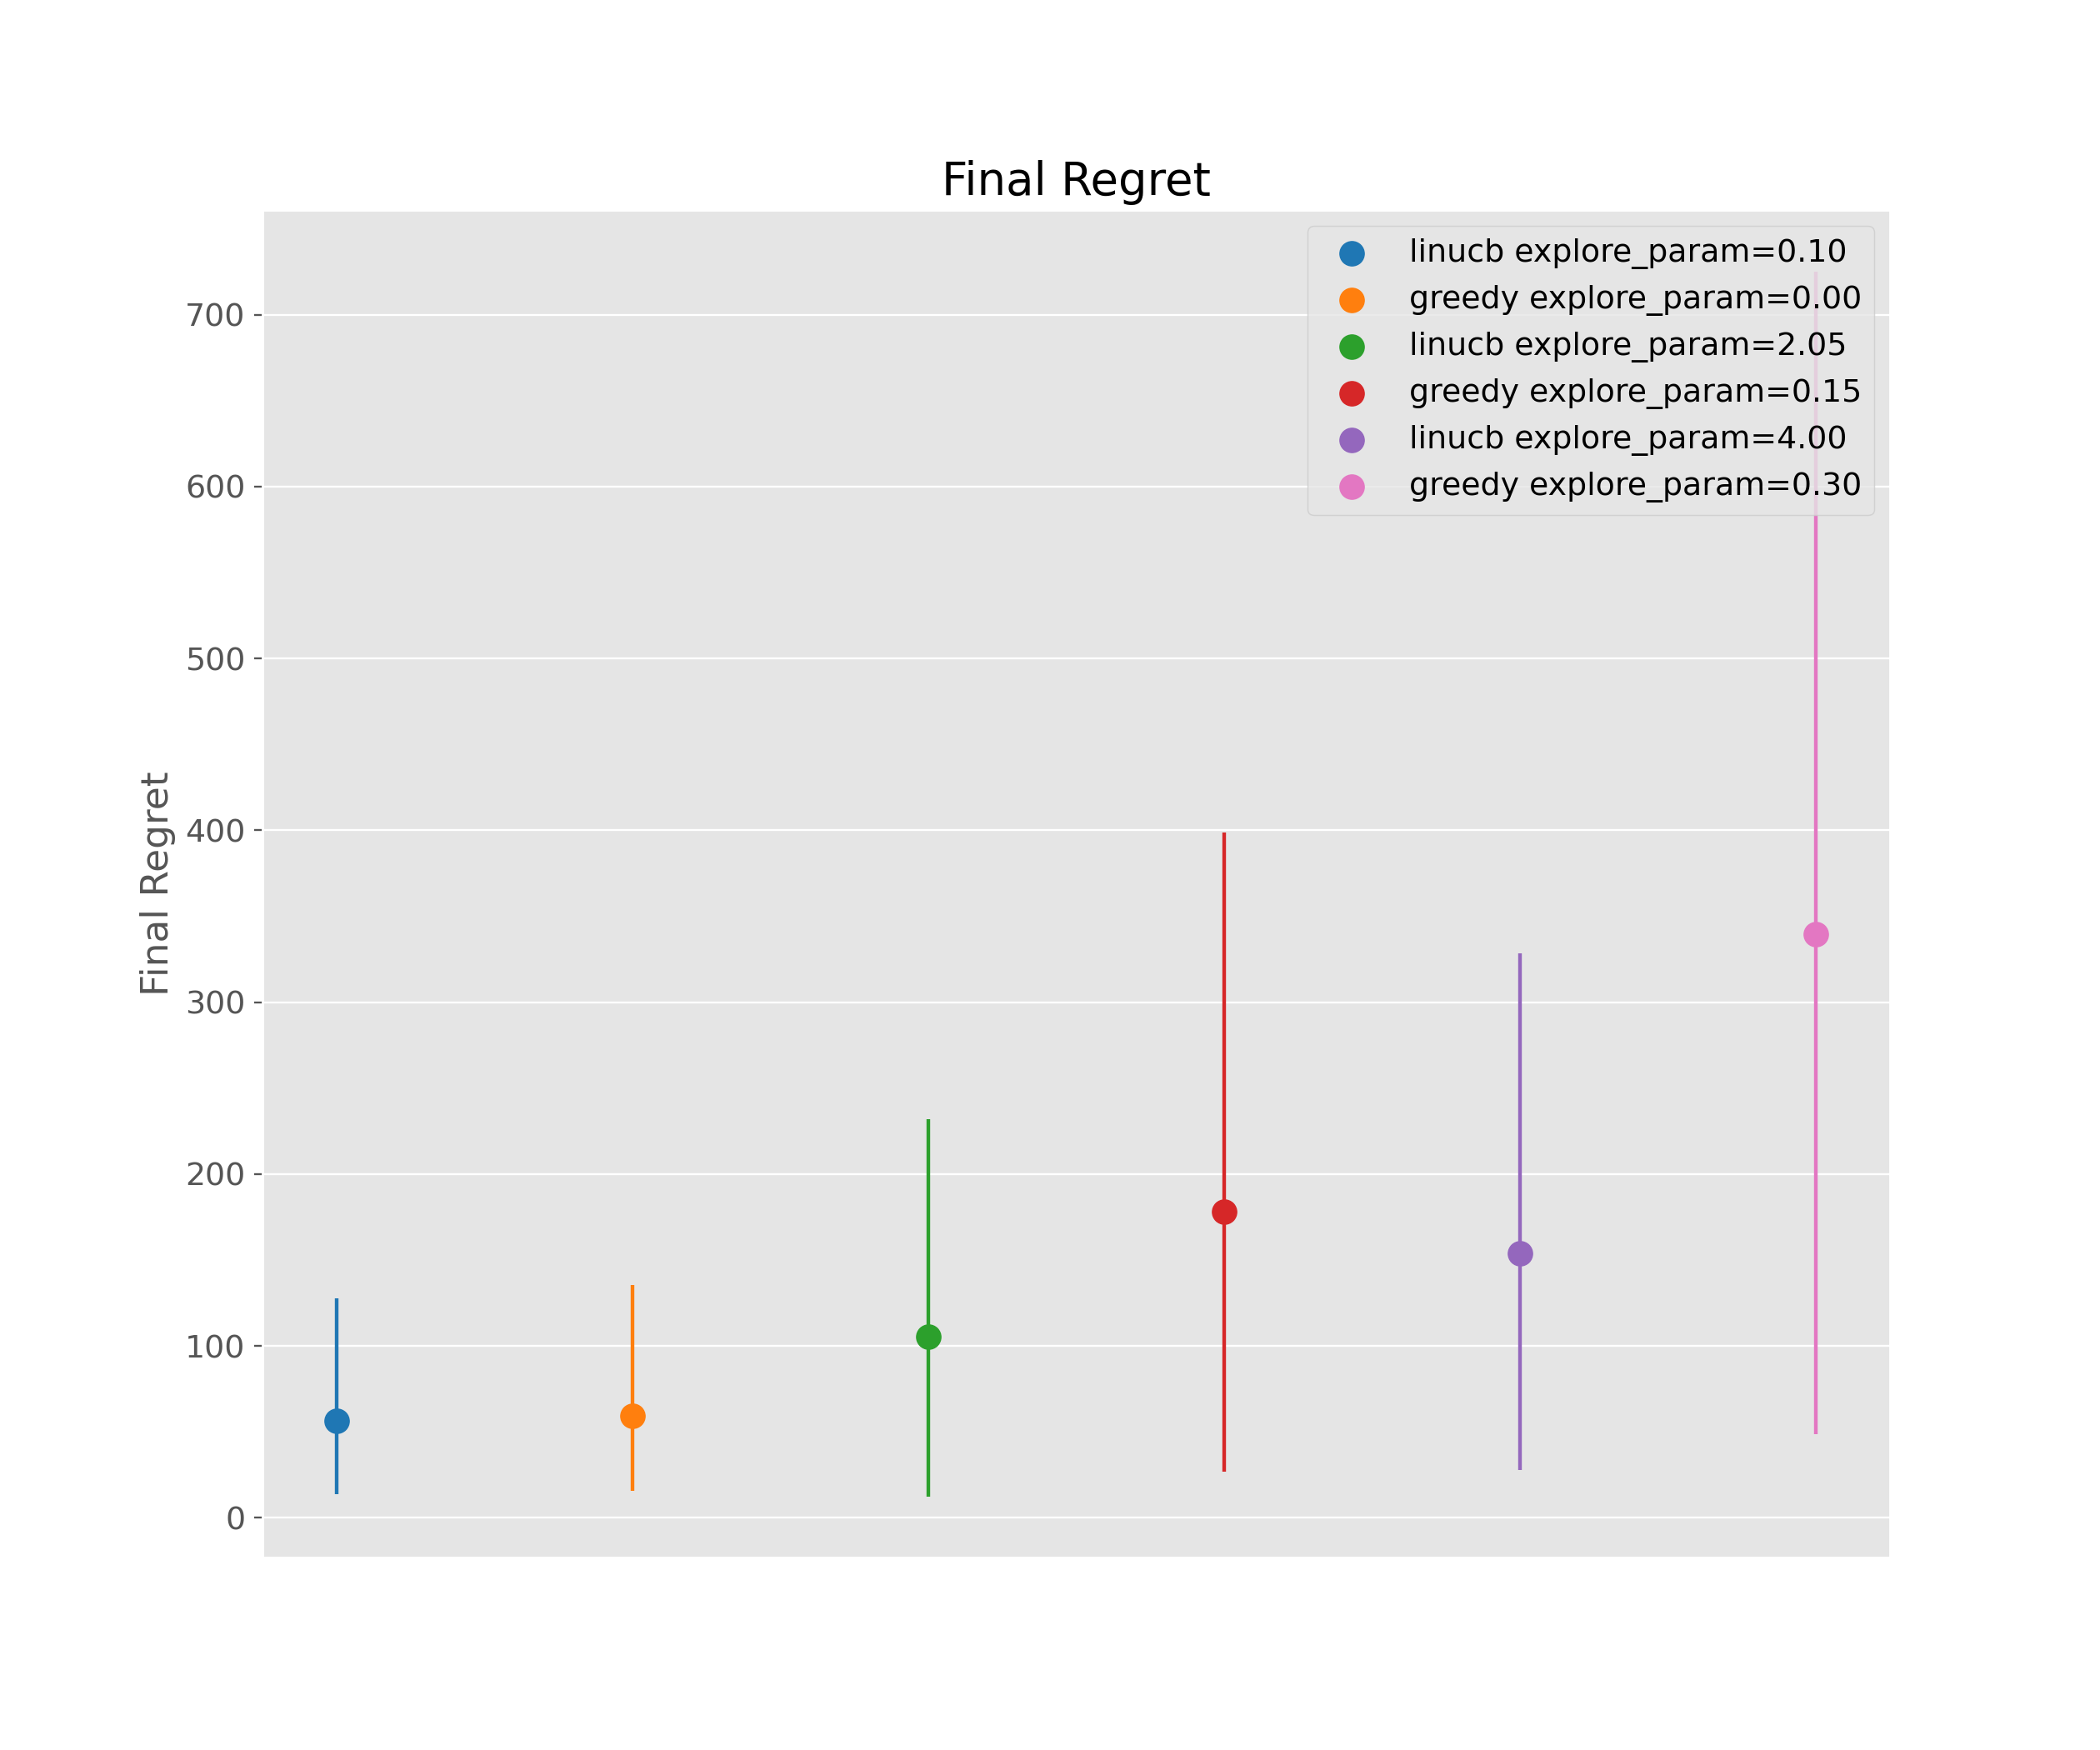
\includegraphics[width=\linewidth]{epsilon_vs_linucb_blobs}
    \caption{Regret without regime change}\label{fig:linucb-blobs-regret-no-regime-change}
  \end{minipage}%
  \begin{minipage}{.45\textwidth}
    \centering
    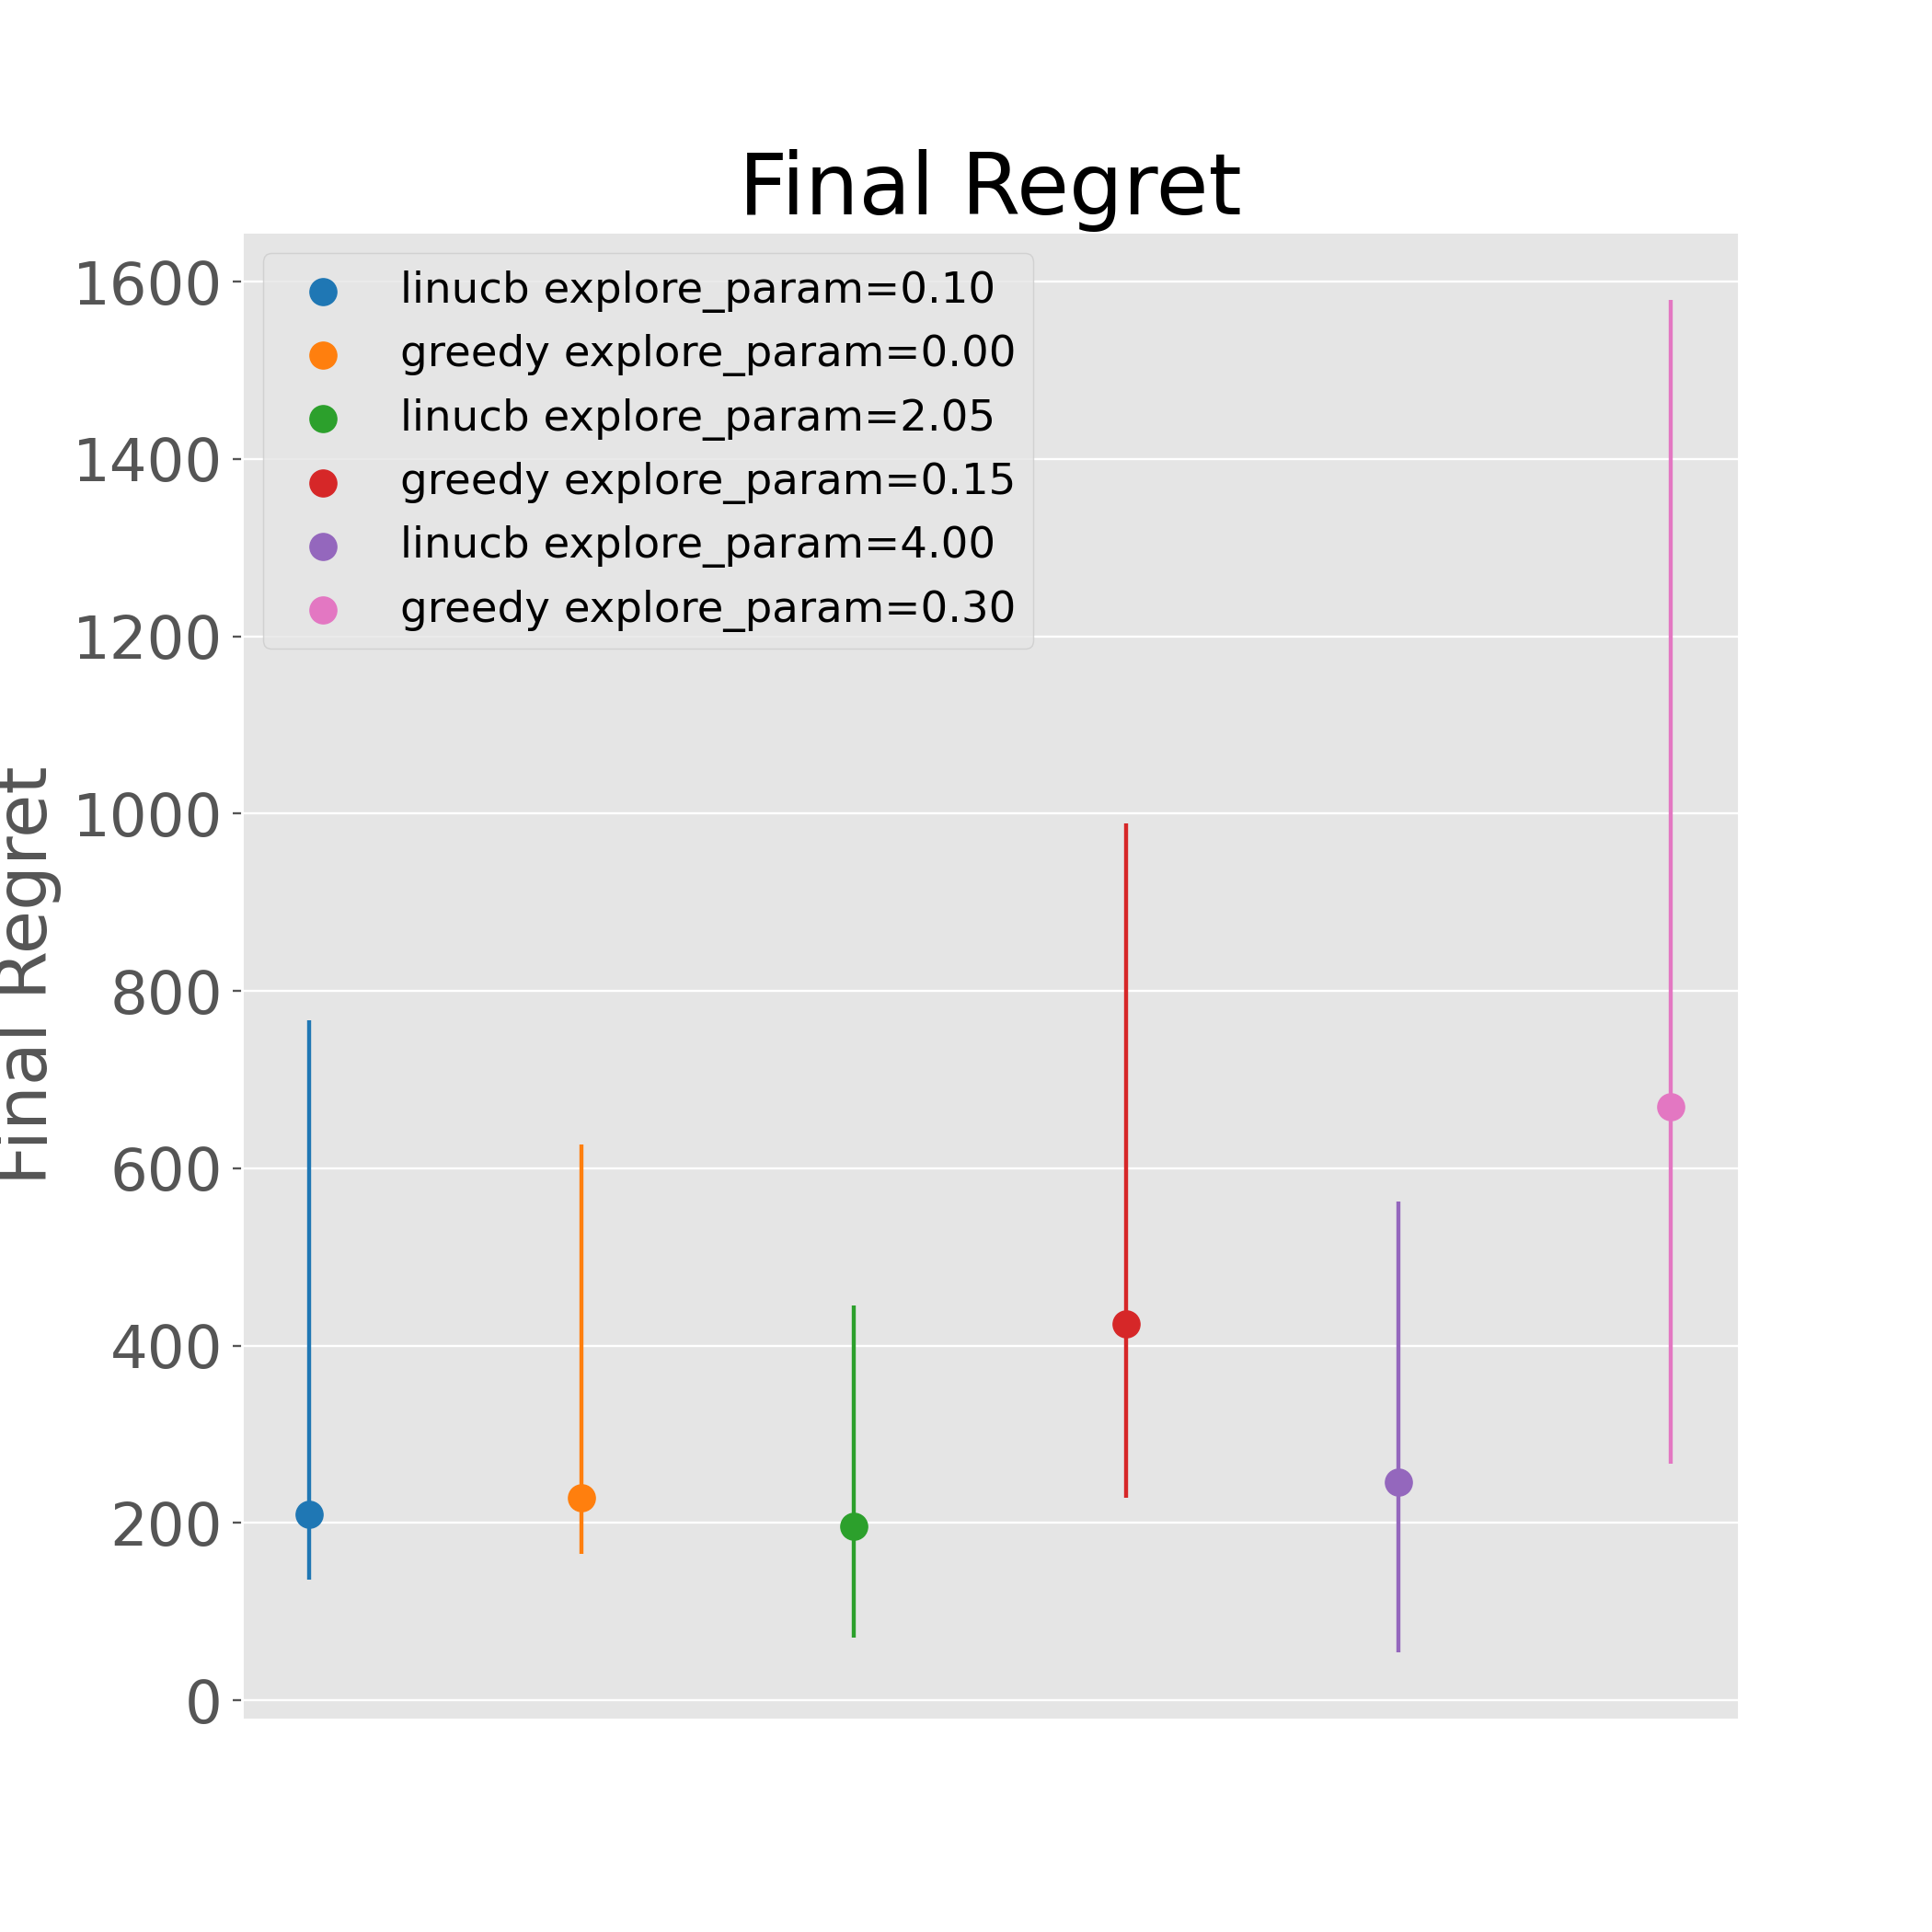
\includegraphics[width=\linewidth]{epsilon_vs_linucb_blobs_regime_change}
    \caption{Regret with regime change}\label{fig:linucb-blobs-regret-regime-change}
  \end{minipage}
\end{figure}


\section{Conclusion}


\bibliography{refs}
\bibliographystyle{plain}

\newpage
\appendix
\section{Appendix}

\subsection{Algorithms omitted from main text}

\begin{algorithm}
  \setstretch{1.2}
    \SetKwInOut{Input}{Input}
    \Input{$\epsilon$ learning rate, $E$ number of epochs, dataset $\{(x_i^{k_i}, y_i^{k_i}, r_i)\}_{i=1}^t$, $b_s$ batch size}

    optimizer $\gets$ SGD($\epsilon, \theta$)\;
    \For{$j = 1, \dots, E$}{
      $\mathcal{D} \gets \{(x_1^{k_1}, y_1^{k_1}, r_1), \dots, (x_t^{k_t}, y_t^{k_t}, r_t)$ \;
      \While{$\mathcal{D}$ is not empty}{
        Sample minibatch $M$ of size $b_s$ from the training examples\;
        $l = \frac{1}{M}\sum_{(x_i^{k_{i}}, y_i^{k_i}, r_i) \in M} (\phi(x_i^{k_{i}}, y_i^{k_i}) - r_i)^2$\;
        $\theta \gets$ update using optimizer with loss $l$\;

        Remove $M$ from $\mathcal{D}$\;
      }
    }
    \caption{Train}\label{algo:train}
  \end{algorithm}


  \begin{algorithm}
  \setstretch{1.2}
    \SetKwInOut{Input}{Input}
    \Input{Rounds $T$ and exploration parameter $\alpha$}
    $A \gets I_{n^2}$\;
    $b \gets 0_{n^2}$\;
    \For{$t \in [T]$}{
      $\theta_t \gets A^{-1}b$
      Observe $K$ pairs of vectors $x^k \in \mathbb{R}^n$, $y^k \in \mathbb{R}^n$\;
      Create $z_{t,k} = (x_1^k, y_1^k, x_1^k, y_1^k, \dots, x_n^k y_{n-1}^k, x_n^k ,y_n^k)$\;
      \For{$k \in [K]$}{
        $p_{t,a} \gets \theta_t^\top z_{t,k} + \alpha \sqrt{z_{t,k}^\top A^{-1} z_{t,a}}$
      }
      Choose action $k_t = \text{argmax}_a p_{t,a}$ with ties broken arbitrarily\;
      Observe payoff $ r_t \in \{-1,1 \}$\;
      $A \gets A + z_{t,k_t}z_{t,k_t}^\top$\;
      $b \gets z_{t,k_t}r_t$\;
    }
    \caption{OnSim-LinUCB}\label{algo:onsim-linucb}
\end{algorithm}

\subsection{Additonal experiments}
\label{sec:additional-experiments}
This section contains additional experiments we ran but omit from the main text due to
space considerations.

\end{document}
